\documentclass[14pt, openany]{report}
\pagestyle{plain}
\usepackage{setspace}
\usepackage{enumitem}
\usepackage[utf8]{inputenc}
\usepackage[T1]{fontenc}
\usepackage{extsizes}
\usepackage[english,russian]{babel}
\let\cdash=\rcdash
\usepackage{geometry}
\usepackage{graphicx}
\graphicspath{ {./images/} }
\usepackage{subcaption}
\usepackage{tempora}
\usepackage[nottoc,notlot,notlof,numbib]{tocbibind}
\usepackage{natbib}
\usepackage{indentfirst}
\usepackage{titlesec}
\titleformat{\chapter}[display]
  {\normalfont\bfseries}{}{0pt}{\Huge}
\usepackage{listings}
\usepackage{xcolor}
\usepackage{hyperref}
\usepackage{tlatex}
\usepackage{url}
\hypersetup{
    colorlinks,
    citecolor=black,
    filecolor=black,
    linkcolor=black,
    urlcolor=black
}

\definecolor{codegreen}{rgb}{0,0.6,0}
\definecolor{codegray}{rgb}{0.5,0.5,0.5}
\definecolor{codepurple}{rgb}{0.58,0,0.82}
\definecolor{backcolour}{rgb}{0.98,0.98,0.98}

\lstdefinestyle{progStyle}{
  frame=tb,
  aboveskip=3mm,
  belowskip=3mm,
  showstringspaces=false,
  columns=flexible,
  basicstyle={\small\ttfamily},
  numbers=none,
  numberstyle=\tiny\color{gray},
  keywordstyle=\color{blue},
  commentstyle=\color{dkgreen},
  stringstyle=\color{green},
  frame=single,
  breaklines=true,
  breakatwhitespace=true,
  tabsize=3,
}

\geometry{
    a4paper,
    left=30mm,
    top=20mm,
    right=20mm,
    bottom=20mm
}
\setlist[itemize]{noitemsep, topsep=0pt}
\setstretch{1.5}
\newcounter{appendix}
\renewcommand{\theappendix}{\Alph{appendix}}

\newcommand{\tlapl}{TLA\textsuperscript{+} }
\newcommand{\prog}[1]{\lstinline[style=progStyle]{#1}}

\title{Применение формальных методов при спецификации бизнес-процессов}
\author{Морковкин Василий}
\date{2022}
\setlength{\parindent}{2em}

\begin{document}
\maketitle
\chapter*{Аннотация}
\par
История отрасли информационных технологий насчитывает немало случаев масштабных нарушений работы из-за изъянов программного обеспечения. Изъяны могут нести финансовые и репутационные потери, а также ставить под угрозу безопасность персональных данных и жизнь человека. Поэтому неотъемлемой частью процесса разработки программного обсепечения является поиск ошибок и их исправление.

Ошибки могут появляться на этапах:
\begin{itemize}
  \item спецификации,
  \item написания кода.
\end{itemize}

Практика покрытия кода автоматизированными тестами помогает минимизировать ошибки этапа написания кода, хорошо описана и широко применяется в индустрии. Ошибки спецификации, однако, такими тестами не обнаруживаются. Они могут проявляться в виде нарушения инваринтов работы системы и даже противоречивости постановки задачи. О возможных противоречиях в требованиях и теоретически достижимых гарантиях любой системы лучше знать еще до начала ее разработки. 

С этой целью данная работа фокусируется на разработке, эксплуатации и анализе применимости метода спецификации бизнес-процессов. За основу берутся формальные методы к верификации. Метод должен осваиваться разработчиками за разумное время, а результат его применения оправдывать расходы на использование.


\setcounter{page}{1}
\tableofcontents
\clearpage



\chapter{Введение}
В данной главе будут введены основные понятия, сформулированы цели, приведен анализ существующих подходов и описана структура работы.

\section{Основные понятия}
В контексте данной работы введем следующие понятия.

\emph{Формальные методы} --- набор математических техник, применяемых в сфере информационных технологий для формализации рассуждений и построения систем с изученными свойствами. 

\emph{Спецификация} --- процесс разработки технического задания, которое может быть транслировано разработчиками в программный код.

\emph{Бизнес-процесс} --- упорядоченный набор действий, выполняемых людьми или машинами, результатом исполнения которых является продукт или услуга, потребляемые пользователями.

\section{Цели работы}

\begin{itemize}
  \item Исследование существующих подходов к валидации спецификаций бизнес-процессов.
  \item Разработка методики спецификации бизнес-процессов с применением формальных методов.
  \item Подготовка инструментария для использования методики в продуктовой разработке.
  \item Применение методики на практике, оценка затрат, преимуществ и ограничений.
\end{itemize}

\section{Актуальность работы}
Ошибки программного обеспечения могут угрожать жизни людей и оборачиваться значительными финансовыми убытками. К примеру, редкая ошибка конкуррентности приводила к неконтролируемому разгону машин Toyota \cite{toyota}. А из-за гонки на данных аппарат лучевой терапии Therac-25 генерировал небезопасные дозы излучения \cite{therac}.

Примеры показывают, что даже инвестиция значительного времени в тестирование продукта не позволяет убедиться в отсутствии ошибок конкурентности. Проблема усугубляется тем, что писать надежные конкурентные тесты - весьма нетривиальная задача \cite{xpConcurrent}. Более того, сам код может соответствовать спецификации, в то время как спецификация может допускать исполнения, ведущие к нежелательным последствиям. 

Дело в том, что люди разрабатывают сложные системы, где число состояний огромно. Занимаясь ручным перебором возможных исполнений легко что-то упустить. Однако, призвав на помощь опыт математиков, о системах можно рассуждать в терминах их свойств. Такие свойства можно формулировать в утверждениях вида:

\begin{itemize}
  \item ``В системе никогда не происходит событие X``,
  \item ``Если произошло X, то в конце концов произойдет и Y``, 
  \item ``Работа алгоритма завершается``, и так далее. 
\end{itemize}

Такие свойства звучат естественно и понятны людям без специальных знаний. Имея механизм проверки этих свойств, можно строить системы, дизайн которых обладает предсказуемым поведением. Подобный подход получил распространение в сфере компьютерной безопасности \cite{formalSecure} и алгоритмов распределенных систем \cite{formalAlg}. 

При разработке бизнес-процессов спецификации зачастую выглядят как текст на натуральном языке (русский, английский и т.д.). В лучшем случае, с применением нотаций вроде BPMN \cite{bpmn} и UML \cite{uml}. Проблема таких спецификаций в том, что они не делают акцент на описании и поддержки инвариантов процессов, которые описывают. На момент написания статьи автору не удалось найти фреймворка, который бы помогал в проверке дизайна на непротиворечивость и отсутствие изъянов, и в то же время был бы доступным для освоения разработчиками или системными аналитиками.
Наверняка, владелец любого продукта не отказался бы от понимания того, что в его системе произойти не может, и что непременно произойдет.
Так почему бы не попробовать формальные методы в продуктовой разработке?


\section{Анализ подходов}
Идея применения формальных методов для спецификации бизнес-процессов не нова. Существующие фреймворки берут на вооружение различные формализмы: \emph{императивный}, \emph{декларативный}, \emph{событийный} и \emph{артефактный}. 

В \emph{императивном} формализме процессы моделируются как множества \emph{задач} или \emph{активностей}, \emph{вентилей (анг. gates)}, и \emph{событий}, связанных \emph{потоками (анг. flows)} или \emph{переходами (анг. transitions)}. Каждая активность описывает единицу работы, а переходы описывают порядок между единицами работы. Императивные подходы включают в себя верификацию распространенных нотаций BPMN \cite{specBPMN}, BPEL \cite{specBPEL}, UML \cite{specUML} и YAWL \cite{specYAWL}. 

С другой стороны, \emph{декларативыный} формализм не прибегает к концепции потоков, которые определяют очередность операций. Вместо этого процесс моделируется как множество \emph{активностей} и множество \emph{ограничений} на очередность этих активностей. Любое исполнение процесса, не запрещенное этими ограничениями, считается корректным.

\emph{Событийный} формализм \cite{specEDC} - еще один подход к моделированию. Его основу составляют \emph{событийные процессные цепочки} --- направленные графы, состоящие из \emph{событий}, \emph{активностей} и \emph{вентилей}. В отличие от императивного подхода, в событийном подходе нет явного моделирования порядка операций.

Наконец, \emph{артефактный} формализм фокусируется на эволюции бизнес-сущностей и данных. Такие спецификации включают в себя понятие жизненного цикла бизнес-сущностей (артефактов), таких как данные.

Для целей работы больше подходит декларативный подход, поскольку он не привязан к конкретной нотации. Более того, его применение не требует уже готовой спецификации. Отталкиваясь от набора простых желаемых свойств, он может выступать в роли интерактивного ассистента при разработке спецификации.


\section{Структура работы}

В Главе 2 рассматриваются математеческие формализмы, пригодные для формирования декларативной методики. Поясняется выбор языка спецификаций \tlapl. Описываются его базовые конструкции и выразительные возможности.

В Главе 3 разрабатывается сама методика. Приводятся детальные примеры использования и анализ опыта реального использования в продуктовой разработке. 

В Глава 4 описывается разработка инструментария \tlapl, полезного для применения методики.

Работа завершается подведением итогов и обсуждением дальнейших путей развития.

\chapter{Выбор инструмента}
В данной главе будет произведен обзор формальных методов \emph{доказательства теорем} и \emph{проверки моделей}, а также пояснен выбор в пользу проверки моделей для целей данной работы. Затем будет обозначена необходимость и способы моделирования времени, проведено сравнение наиболее популярных инструментов проверки моделей \emph{Alloy} и \tlapl. И, наконец, описаны концепты \tlapl, которые будут использоваться в дальнейшем.

\section{Сравнение технологий}
В плеаде формальных методов ярко выделяются два похода: \emph{доказательство теорем (анг. theorem proving)} и \emph{проверка моделей (анг. model checking)}. 

В доказательстве теорем верификация устроена индуктивно, шаг за шагом: отталкиваясь от выбранной системы аксиом и правил вывода выводятся комплексные утверждения. При использовании доказательного ассистента нам доступна работа с более точными представлениями наших систем. Однако, занимаясь проблемой разрешимости (нем. Entscheidungsproblem), Алан Тьюринг показал \cite{turing}, что не может существовать завершающегося алгоритма, который бы в качестве входных данных принимал утверждение некоторого формального языка, а на выходе выдавал бы один из двух ответов: ``истина`` или ``ложь``. Следствием этого фундаментального результата является необходимость проводить доказательства вручную (за исключением ограниченного набора простых случаев), а это требует значительной экспертизы.

В подходе проверки моделей мы описываем абстрактную версию системы и можем автоматически (с помощью \emph{проверщика моделей (анг. model checker)}) проверить ее на соответствие свойствам. При этом наша модель должна быть достаточно маленькой (в терминах количества состояний), чтобы быть обработанной проверщиком за разумное время.

Поскольку нашей целью является создание методики, доступной для освоения широким кругом людей без должной математической подготовки, фундаментом методики послужит \emph{проверка моделей}.

\section{Моделирование времени}
Нам интересна проверка утверждений вида ``X всегда верно``, ``В конце концов X будет верно``, ``X верно до тех пор, пока не верно Y``, ``Если X, то в конце концов Y будет врно``. Эти утверждения строятся вокруг концепта времени. Значит, нужен способ для его моделирования. Подходящим формализмом является \emph{темпоральная логика}. Ее разновидность, \emph{линейная темпоральная логика}, как раз позволяет кодировать утверждения о будущих путях исполнения. Типичными операторами являются: 


\begin{itemize}
  \item всегда \((\Box F)\)
  \item в итоге \((\Diamond F)\)
  \item если было \(P\), то будет и \(Q\) \((P \leadsto Q)\)
\end{itemize}


Наиболее развитыми языками спецификаций с возможностями проверки моделей и рассуждения о времени с помощью линейной темпоральной логики являются \tlapl \cite{tla} и Alloy версии 6 \cite{alloy}.

На момент написания в Alloy поддержка темпоральной логики появилась недавно, не покрыта документацией и примерами использования. Поэтому, хоть Alloy и является перспективным инструментом верификации с акцентом на визуализацию, в данной работе будет использоваться \tlapl.

\section{Требуемый функционал \tlapl}
Большинство математических концептов, используемых в \tlapl, просты. Данная секция дает представление о том, какие возможности языка будут использованы для реализации методики методики. 

Зачастую языки программирования имеют свою нотацию для математических оперторов. Например, логические операторы Java (\(!, \&\&, ||\)) в математике обозначаются как (\(\neg, \lor, \land\)) и отсутствует на большинстве раскладок клавиатур. По этой причине логический операторы в \tlapl записываются как (\char`~, /\char`\\, \char`\\/). Для других математических символов используются их эквиваленты из LaTeX.

\subsection{Логика высказываний}

\tlapl строится поверх \emph{логики высказываний}. Высказывание --- это утверждение на булевых переменных, которые принимают значения True или False. К примеру, выражение 
\[A \land (B \lor \neg C)\]
означает ``A верно И (B верно ИЛИ С ложно)``, а выражение
\[A \Rightarrow B = \neg A \lor B\]
называется ``импликацией`` и эквивалентно утверждению ``либо A ложно, либо B истинно``. Равенство в логике высказываний определяется как импликация в обе стороны.

\tlapl умеет вычислять высказывания:
\begin{tla}
  Q: FALSE => FALSE
  A: TRUE
\end{tla}
\begin{tlatex}
\@x{\@s{8.2} Q \.{:} {\FALSE} \.{\implies} {\FALSE}}%
\@x{\@s{8.2} A\@s{1.69} \.{:} {\TRUE}}%
\end{tlatex}

\begin{tlatex}
\@x{\@s{8.2} Q \.{:} {\FALSE} \.{\implies} {\FALSE}}%
\@x{\@s{8.2} A\@s{1.69} \.{:} {\TRUE}}%
\end{tlatex}

Например, используя генераторы множеств, можно вывести таблицу истинности для импликации:

\begin{tla}
  Q: {<<A, B, A => B>>: A,B \in BOOLEAN}
  A: {<<FALSE, FALSE, TRUE>>,
      <<FALSE, TRUE, TRUE>>,
      <<TRUE, FALSE, FALSE>>,
      <<TRUE, TRUE, TRUE>>}
\end{tla}
\begin{tlatex}
 \@x{\@s{8.2} Q \.{:} \{ {\langle} A ,\, B ,\, A \.{\implies} B {\rangle}
 \.{:} A ,\, B \.{\in} {\BOOLEAN} \}}%
 \@x{\@s{8.2} A\@s{1.69} \.{:} \{ {\langle} {\FALSE} ,\, {\FALSE} ,\, {\TRUE}
 {\rangle} ,\,}%
\@x{\@s{39.24} {\langle} {\FALSE} ,\, {\TRUE} ,\, {\TRUE} {\rangle} ,\,}%
\@x{\@s{39.24} {\langle} {\TRUE} ,\, {\FALSE} ,\, {\FALSE} {\rangle} ,\,}%
\@x{\@s{39.24} {\langle} {\TRUE} ,\, {\TRUE} ,\, {\TRUE} {\rangle} \}}%
\end{tlatex}

\subsection{Теория множеств}
Следующим важным формализмом \tlapl является \emph{теория множеств}. Несколько примеров:
\begin{itemize}
  \item \(\{1, 2\}\) - фигурные скобки в качестве конструктора,
  \item \(1..N\) - множество от 1 до N,
  \item \(x \in S\) - проверка принадлежности x множеству S,
  \item \(S  \times S\) - декартово произведение множества S с самим собой.
\end{itemize}

Множества можно фильтровать. Выражение \(\{x \in S: P(x)\}\) является множеством всех элементов \(S\), для которых истин предикат \(P(x)\):

\begin{tla}
   Q: {<<x, y>> \in {1,2} \X {3,4}: x > y}
   A: {<<1, 3>>, <<1, 4>>, <<2, 3>>, <<2, 4>>}
\end{tla}
\begin{tlatex}
 \@x{\@s{12.29} Q \.{:} \{ {\langle} x ,\, y {\rangle} \.{\in} \{ 1 ,\, 2 \}
 \.{\times} \{ 3 ,\, 4 \} \.{:} x \.{>} y \}}%
 \@x{\@s{12.29} A\@s{1.69} \.{:} \{ {\langle} 1 ,\, 3 {\rangle} ,\, {\langle}
 1 ,\, 4 {\rangle} ,\, {\langle} 2 ,\, 3 {\rangle} ,\, {\langle} 2 ,\, 4
 {\rangle} \}}%
\end{tlatex}

Элементы множества можно преобразовывать. Выражение \(\{P(x): x \in S\}\) применяет \(P\) к каждому элементу:
\begin{tla}
  Q: {x * x: x \in 1..3}
  A: {1, 4, 9}
\end{tla}
\begin{tlatex}
\@x{\@s{8.2} Q \.{:} \{ x \.{*} x \.{:} x \.{\in} 1 \.{\dotdot} 3 \}}%
\@x{\@s{8.2} A\@s{1.69} \.{:} \{ 1 ,\, 4 ,\, 9 \}}%
\end{tlatex}

Полезным также бывает оператор выбора \(CHOOSE~x \in S: P(x)\), который выбирает случайный элемент множества \(S\), удовлетворяющий предикату \(P\). Стоит отметить, что проверщик моделей не будет выполнять полный перебор возможных вариантов выбора, а зафиксирует один.
\begin{tla}
  Q: CHOOSE x \in 1..100: x > 42
  A: 43
\end{tla} 
\begin{tlatex}
\@x{\@s{8.2} Q \.{:} {\CHOOSE} x \.{\in} 1 \.{\dotdot} 100 \.{:} x \.{>} 42}%
\@x{\@s{8.2} A\@s{1.69} \.{:} 43}%
\end{tlatex}

Ожидаемо присутствуют следующие операторы:
\begin{tla}
  Q: {} \in {{}}
  A: TRUE
  Q: {} \notin {{}}
  A: FALSE
  Q: {1,2} \subseteq {1,2,3}
  A: TRUE
  Q: {1,2} \union {3}
  A: {1,2,3}
  Q: {1,2} \intersect {2, 3}
  A: {2}
  Q: {1, 2} \ {2, 3}
  A: {1}
  Q: SUBSET {1,2}
  A: {{}, {1}, {2}, {1,2}}
  Q: UNION {{1}, {2}}
  A: {1, 2}
\end{tla}
\begin{tlatex}
\@x{\@s{8.2} Q \.{:} \{ \} \.{\in} \{ \{ \} \}}%
\@x{\@s{8.2} A\@s{1.69} \.{:} {\TRUE}}%
\@x{\@s{8.2} Q \.{:} \{ \} \.{\notin} \{ \{ \} \}}%
\@x{\@s{8.2} A\@s{1.69} \.{:} {\FALSE}}%
\@x{\@s{8.2} Q \.{:} \{ 1 ,\, 2 \} \.{\subseteq} \{ 1 ,\, 2 ,\, 3 \}}%
\@x{\@s{8.2} A\@s{1.69} \.{:} {\TRUE}}%
\@x{\@s{8.2} Q \.{:} \{ 1 ,\, 2 \} \.{\cup} \{ 3 \}}%
\@x{\@s{8.2} A\@s{1.69} \.{:} \{ 1 ,\, 2 ,\, 3 \}}%
\@x{\@s{8.2} Q \.{:} \{ 1 ,\, 2 \} \.{\cap} \{ 2 ,\, 3 \}}%
\@x{\@s{8.2} A\@s{1.69} \.{:} \{ 2 \}}%
\@x{\@s{8.2} Q \.{:} \{ 1 ,\, 2 \} \.{\,\backslash\,} \{ 2 ,\, 3 \}}%
\@x{\@s{8.2} A\@s{1.69} \.{:} \{ 1 \}}%
\@x{\@s{8.2} Q \.{:} {\SUBSET} \{ 1 ,\, 2 \}}%
 \@x{\@s{8.2} A\@s{1.69} \.{:} \{ \{ \} ,\, \{ 1 \} ,\, \{ 2 \} ,\, \{ 1 ,\, 2
 \} \}}%
\@x{\@s{8.2} Q \.{:} {\UNION} \{ \{ 1 \} ,\, \{ 2 \} \}}%
\@x{\@s{8.2} A\@s{1.69} \.{:} \{ 1 ,\, 2 \}}%
\end{tlatex}


\subsection{Логика предикатов}
Комбинация логики высказываний и теории множеств дает логику предикатов, которая позволяет писать утверждения об элементах множества и является базисом разработки на \tlapl. Логика предикатов добавляет кванторы существования (\(\exists\)) и всеобщности (\(\forall\)):

\begin{tla}
  Q: \E x \in {1,2}: x < 0
  A: FALSE
  Q: \A x \in {1,2}: x > 0
  A: TRUE
\end{tla}
\begin{tlatex}
\@x{\@s{8.2} Q \.{:} \E\, x \.{\in} \{ 1 ,\, 2 \} \.{:} x \.{<} 0}%
\@x{\@s{8.2} A\@s{1.69} \.{:} {\FALSE}}%
\@x{\@s{8.2} Q \.{:} \A\, x \.{\in} \{ 1 ,\, 2 \} \.{:} x \.{>} 0}%
\@x{\@s{8.2} A\@s{1.69} \.{:} {\TRUE}}%
\end{tlatex}

\subsection{Моделирование данных}
Помимо множеств для моделирования данных в \tlapl используются \emph{кортежи} и \emph{структуры}.

Кортежи - упорядоченные последовательности элементов произвольного типа. Основные операторы над ними:
\begin{tla}
  Q: Head(<<0,"A">>)
  A: 0
  Q: Tail(<<0,"A">>)
  A: <<"A">>
  Q: Append(<<0>>, "A")
  A: <<0, "A">>
  Q: <<0>> \o <<"A">> 
  A: <<0, "A">>
  Q: Len(<<0,"A",TRUE>>)
  A: 3
  Q: DOMAIN <<"One", "Two">> 
  A: {1, 2}
\end{tla}
\begin{tlatex}
\@x{\@s{8.2} Q \.{:} Head ( {\langle} 0 ,\,\@w{A} {\rangle} )}%
\@x{\@s{8.2} A\@s{1.69} \.{:} 0}%
\@x{\@s{8.2} Q \.{:} Tail ( {\langle} 0 ,\,\@w{A} {\rangle} )}%
\@x{\@s{8.2} A\@s{1.69} \.{:} {\langle}\@w{A} {\rangle}}%
\@x{\@s{8.2} Q \.{:} Append ( {\langle} 0 {\rangle} ,\,\@w{A} )}%
\@x{\@s{8.2} A\@s{1.69} \.{:} {\langle} 0 ,\,\@w{A} {\rangle}}%
 \@x{\@s{8.2} Q \.{:} {\langle} 0 {\rangle} \.{\circ} {\langle}\@w{A}
 {\rangle}}%
\@x{\@s{8.2} A\@s{1.69} \.{:} {\langle} 0 ,\,\@w{A} {\rangle}}%
\@x{\@s{8.2} Q \.{:} Len ( {\langle} 0 ,\,\@w{A} ,\, {\TRUE} {\rangle} )}%
\@x{\@s{8.2} A\@s{1.69} \.{:} 3}%
\@x{\@s{8.2} Q \.{:} {\DOMAIN} {\langle}\@w{One} ,\,\@w{Two} {\rangle}}%
\@x{\@s{8.2} A\@s{1.69} \.{:} \{ 1 ,\, 2 \}}%
\end{tlatex}

Структуры являются ассоциативными массивами и конструируются конутсрукциями вида \([k1 \mapsto v1, k2 \mapsto v2]\):
\begin{tla}
  Q: q == [x |-> {}, y |-> {0, "A"}]
     q.y
  A: {0, "A"}
  Q: DOMAIN q
  A: {"x", "y"}
\end{tla}
\begin{tlatex}
 \@x{\@s{8.2} Q \.{:} q \.{\defeq} [ x \.{\mapsto} \{ \} ,\, y \.{\mapsto} \{
 0 ,\,\@w{A} \} ]}%
\@x{\@s{32.04} q . y}%
\@x{\@s{8.2} A\@s{1.69} \.{:} \{ 0 ,\,\@w{A} \}}%
\@x{\@s{8.2} Q \.{:} {\DOMAIN} q}%
\@x{\@s{8.2} A\@s{1.69} \.{:} \{\@w{x} ,\,\@w{y} \}}%
\end{tlatex}

Определен синтаксис генераторов структур:

\begin{tla}
  Q: [x : {1}, y : {0, 1}]
  A: {[x |-> 1, y |-> 0], [x |-> 1, y |-> 1]}
\end{tla}
\begin{tlatex}
\@x{\@s{8.2} Q \.{:} [ x \.{:} \{ 1 \} ,\, y \.{:} \{ 0 ,\, 1 \} ]}%
 \@x{\@s{8.2} A\@s{1.69} \.{:} \{ [ x \.{\mapsto} 1 ,\, y \.{\mapsto} 0 ] ,\,
 [ x \.{\mapsto} 1 ,\, y \.{\mapsto} 1 ] \}}%
\end{tlatex}


\subsection{Операторы и функции}
Для манипуляции данными используются \emph{операторы} и \emph{функции}.

Операторы \tlapl похожи на функции в обычных языках программирования:

\begin{tla}
  Q: IsPrime(x) == x > 1 /\ ~\E d \in 2..x-1: x % d = 0
     IsPrime(37)
  A: TRUE
\end{tla}
\begin{tlatex}
 \@x{\@s{8.2} Q \.{:} IsPrime ( x ) \.{\defeq} x \.{>} 1 \.{\land} {\lnot}
 \E\, d \.{\in} 2 \.{\dotdot} x \.{-} 1 \.{:} x \.{\%} d \.{=} 0}%
\@x{\@s{32.04} IsPrime ( 37 )}%
\@x{\@s{8.2} A\@s{1.69} \.{:} {\TRUE}}%
\end{tlatex}

Функции же больше похожи на словари, где ключи лежат в некотором множестве определения, а значения в множестве значений:

\begin{tla}
  Q: Squares[x \in 1..4] == x * x
     Squares[4]
  A: 16
  Q: DOMAIN Squares
  A: {1, 2, 3, 4}
\end{tla}
\begin{tlatex}
 \@x{\@s{8.2} Q \.{:} Squares [ x \.{\in} 1 \.{\dotdot} 4 ] \.{\defeq} x \.{*}
 x}%
\@x{\@s{32.04} Squares [ 4 ]}%
\@x{\@s{8.2} A\@s{1.69} \.{:} 16}%
\@x{\@s{8.2} Q \.{:} {\DOMAIN} Squares}%
\@x{\@s{8.2} A\@s{1.69} \.{:} \{ 1 ,\, 2 ,\, 3 ,\, 4 \}}%
\end{tlatex}

На самом деле кортежи и структуры реализованы поверх функций. В случае кортежей областью определения являются натуральные чилса.

\subsection{PlusCal}
Для удобства разработчиков был создан язык PlusCal, код которого пишется в многострочных комментариях и транспилируется в \tlapl. Язык похож на C и предоставляет привычные выражения контроля, такие как \emph{while}, \emph{if-then-else}, \emph{goto}. Полезено выражение \(with~x \in S\), которое позволяет указать проверщику моделей, что нужно перебрать все возможные значения \(x\) из множества \(S\).

Пример типичного кода на PlusCal:
\begin{ppcal}
  --algorithm counter
  variables x = 0
  begin
    while x < 5 do
      with inc \in {1, 2} do
        x := x + inc
      end with;
    end while;
  end algorithm; 
\end{ppcal}
\begin{tlatex}
\@x{\@s{8.2} {\p@mmalgorithm} counter}%
\@x{\@s{8.2} {\p@variables} x \.{=} 0}%
\@x{\@s{8.2} {\p@begin}}%
\@x{\@s{16.4} {\p@while} x \.{<} 5 {\p@do}}%
\@x{\@s{24.59} {\p@with} inc \.{\in} \{ 1 ,\, 2 \} {\p@do}}%
\@x{\@s{32.8} x \.{:=} x \.{+} inc}%
\@x{\@s{24.59} {\p@end} {\p@with} {\p@semicolon}}%
\@x{\@s{16.4} {\p@end} {\p@while} {\p@semicolon}}%
\@x{\@s{8.2} {\p@end} {\p@algorithm} {\p@semicolon}}%
\end{tlatex}

\subsection{Темпоральная логика}
Выше уже упоминались операторы темпоральной логики. Они позволяют нам определять свойства \emph{живости (анг. liveness)}, которые описывают, что же должно обязательно происходить в нашей системе со временем.

Попробуем запустить проверку примера выше на соответствие различным темпоральным свойствам и посмотрим на результат:

\begin{itemize}
  \item 
    \begin{tla} 
      [](x > 0)
    \end{tla}
\begin{tlatex}
\@x{\@s{24.59} {\Box} ( x \.{>} 0 )}%
\end{tlatex}
: \(x\) всегда больше нуля. Успех проверки.
  \item
    \begin{tla}
      <>(x = 5)
    \end{tla}
\begin{tlatex}
\@x{\@s{24.59} {\Diamond} ( x \.{=} 5 )}%
\end{tlatex}
: \(x\) обязательно будет равен 5. Поскольку наш счетчик уменьшается или на 1, или на 2, проверщик находит исполнение, в котором свойство не выполняется: \(0,2,4,6\). Свойство не выполняется.
  \item
    \begin{tla}
      (x = 0) ~> (x > 3)
    \end{tla}
\begin{tlatex}
\@x{\@s{24.59} ( x \.{=} 0 ) \.{\leadsto} ( x \.{>} 3 )}%
\end{tlatex}
: если значение \(x\) было 0, то обязательно будет больше 3. Успех проверки.
\end{itemize}

Как видно, знания базовых элементов математики вроде теории множеств почти достаточно для использования \tlapl. Новым для разработчиков может стать формализм темпоральной логики, однако и он прост в изучении, поскольку строится на интуитивном понимании событийности. Также язык предоставляет привычные разработчикам управляющие конструкции. Основываясь на сказанном, язык спецификаций \tlapl составит основу разрабатываемой методики.


\chapter{Методика}
В данной главе приводятся рассуждения на тему наиболее популярных вариантов специфицирования бизнес-процессов. Затем с опором на это разрабатывается методика специфицирования, состоящая из этапов уточнения требований, написания спецификации, ее эволюции со временем и поддержки. Наконец, приводятся примеры применения и анализ применимости, основанный на опыте использования.

\section{Языки и нотации}
От сложившихся процессов и состава сотрудников отдела разработки зависит и процесс спецификации. Проведем классификацию этого процесса по возрастанию комплексности подхода:
\begin{itemize}
  \item Требования формулируются владельцем продукта. Зачастую в устном виде.
  \item Для формулирования привлекается бизнес-аналитика. Постановки записаны на естественных языках (русском, английском и т.д.). Определены мотивация, цели и критерии готовности (анг. DOD - definition of done).
  \item Для формулирования помимо бизнес-аналитики привлекается системная аналитика. Спецификации могут быть снабжены диаграммами в таких нотация как, UML \cite{uml} и BPMN \cite{uml}. Конечно, существуют и другие нотации (например, такие как BPEL \cite{bpel} и YAWL \cite{yawl}), однако они не так распространены.

Используя формальные методы, мы насыщаем спецификацию \emph{семантикой}, которая отсутствует как в естественных языках, так и в перечисленных нотациях. Однако, чтобы приступить к этому, нам необходимо лучше выяснить нужные бизнесу инварианты.

\end{itemize}

\section{Уточнение требований}
Рабочий способ ``конденсации`` инвариантов для нашей формальной спецификации --- через общение с визионерами продукта. Эти люди хорошо понимают пользователей и цену ошибки. При выяснении требований полезно задавать следующие вопросы в контексте специфицируемого процесса:
\begin{itemize}
  \item Когда можно считать процесс успешно завершенным?
  \item Что может нанести ущерб клиенту?
  \item Из-за чего клиент может испытать раздражение?
  \item Что может принести нам финансовые убытки?
  \item Что может нанести нам репутационный ущерб?
  \item Есть ли требования от регулятора?
\end{itemize}

Ответы на эти вопросы помогают понять, что важно бизнесу и клиенту, чего происходить не должно и что обязательно должно произойти. Собрав такие свойства, мы подходим непосредственно к этапу формальной спецификации.

\section{Спецификация}
Одним из преимуществ того, что \tlapl --- язык спецификации, являетсято, что его операторы могут обладать намного большей выразительной силой, чем функции в обычных программах. Это также является и недостатком: если спецификация использует ``слишком выразительный`` оператор, она не может быть напрямую транслирована в код. Обычно это нормально: разрабатывая код для большой системы мы вряд беспокоймся о том, корректна ли наша функция сортировки.

Чтобы процесс спецификации с применением \tlapl был доступен для повседневного применения, нам необходимо исследовать возможные подходы, ``строительные блоки``, от которых можно отталкиваться. 

\subsection{Алгоритм}
Выделем первый класс процессов: \emph{алгоритмы}. Под алгоритмом будем подразумевать процессы, которые должны завершаться и выдавать результат (в отличие от процессов, которые идут бесконечно и непрерывно взаимодействуют с окружением).

В свою очередь алгоритмы можно разделить на \emph{однопроцессные} и \emph{многопроцессные}. В контексте алгоритма под процессом понимается актор алгоритма, уместна аналогия с системными процессами.

\subsubsection{Однопроцессный}

Большинство однопроцессных алгоритмов можно свести к описанию по следующему шаблону:
\begin{ppcal}
  --algorithm singleProcess
    variables
      input = ...
      result;
    define
      Expected(input) == ...
    end define;
    begin
      \* // имплементация
      assert output = Expected(input);
    end algorithm;
\end{ppcal}
\begin{tlatex}
\@x{\@s{8.2} {\p@mmalgorithm} singleProcess}%
\@x{\@s{16.4} {\p@variables}}%
\@x{\@s{24.59} input \.{=} \.{\dots}}%
\@x{\@s{24.59} result {\p@semicolon}}%
\@x{\@s{16.4} {\p@define}}%
\@x{\@s{24.59} Expected ( input ) \.{\defeq} \.{\dots}}%
\@x{\@s{16.4} {\p@end} {\p@define} {\p@semicolon}}%
\@x{\@s{16.4} {\p@begin}}%
\@x{\@s{24.59}}%
\@y{%
  // имплементация
}%
\@xx{}%
\@x{\@s{24.59} {\p@assert} output \.{=} Expected ( input ) {\p@semicolon}}%
\@x{\@s{16.4} {\p@end} {\p@algorithm} {\p@semicolon}}%
\end{tlatex}

Оператор \emph{Expected} --- то, что мы на самом деле пытаемся реализовать: он берет некоторые входные данные и возвращает значение, которое должен производить алгоритм, если он корректен. Помимо него в блоке \emph{define} могут быть определены любые операторы, которые могут использоваться алгоритмом и которые мы не планируем здесь верифицировать. Далее следует код алгоритма на PlusCal, который мы хотим проверить на работоспособность на заданном множестве входных данных. Алгоритм сохраняет результат своей работы в переменную \emph{output}, которой мы намеренно не дали начального значения. Также в секцию \emph{variables} должны быть помещены любые переменные, нужные алгоритму, поскольку в теле алгоритма новые объявления невозможны. В конце происходит проверка на соответствие вывода алгоритма и ожидаемого результата.

Безусловно, шаблон не является строгим. Если алгоритм сложен, мы можем выносить новые процедуры и макросы, чтобы разбить его на части.

Спецификации однопроцессных алгоритмов могут напоминать \emph{тестирование на основе модели (анг. property-based testing)}. Однако, здесь имеется отличие в уровне абстракции. В то время как тестирование применяется к конкретному коду, в спецификации мы можем этот уровень выбрать по нашему усмотрению.

\subsubsection{Многопроцессный}

Многопроцессные алгоритмы похожи на однопроцессные, кроме того что в них мы также хотим проверять, что все процессы завершатся. Вместо прямого кодирования выражения assert мы запишем это как свойство живучести (анг. liveness). Это означает использование оператора ``в конце концов всегда`` (\(\Diamond \Box\)), который проверяет, что алгоритм завершается с некоторым истинным условием в конце.

Шаблон для таких алгоритмов выглядит следующим образом:

\begin{ppcal}
  --algorithm singleProcess
    variables
      input = ...
    define
      Success == <>[](someProperty)
      
    end define;

    fair process proc \in 1..N
    variables ...;
    begin
      \* // имплементация
    end process;

    end algorithm;
\end{ppcal}
\begin{tlatex}
\@x{\@s{8.2} {\p@mmalgorithm} singleProcess}%
\@x{\@s{16.4} {\p@variables}}%
\@x{\@s{24.59} input \.{=} \.{\dots}}%
\@x{\@s{16.4} {\p@define}}%
\@x{\@s{24.59} Success \.{\defeq} {\Diamond} {\Box} ( someProperty )}%
\@pvspace{8.0pt}%
\@x{\@s{16.4} {\p@end} {\p@define} {\p@semicolon}}%
\@pvspace{8.0pt}%
\@x{\@s{16.4} {\p@fair} {\p@process} proc \.{\in} 1 \.{\dotdot} N}%
\@x{\@s{16.4} {\p@variables} \.{\dots} {\p@semicolon}}%
\@x{\@s{16.4} {\p@begin}}%
\@x{\@s{24.59}}%
\@y{%
  // имплементация
}%
\@xx{}%
\@x{\@s{16.4} {\p@end} {\p@process} {\p@semicolon}}%
\@pvspace{8.0pt}%
\@x{\@s{16.4} {\p@end} {\p@algorithm} {\p@semicolon}}%
\end{tlatex}

Процессы в PlusCal можно моделировать с помощью специальной конструкции \emph{process}. У каждого процесса должен быть свой индивидуальный идентификатор, который присваевается в блоке \(\in 1..N\). Для запуска необходимо указать проверщику, что формула \emph{Success} это свойство, которое необходимо проверять.

Надо сказать, что в чистом виде этих шаблонов обычно недостаточно для написания спецификации. Однако вместе со следующим подходом они дают хороший результат.

\subsection{Автомат}
Как упоминалось выше, спецификации выразительнее, чем код, и за это есть своя цена: не всегда очевидно, как перейти от спецификации к реальности. Решением этой проблемы является подход, в котором мы пишем максимально абстрактную спецификацию и наполняем ее деталями в нужных местах, которые ближе к реализации в реальном коде. Для этого можно использовать паттерн \emph{автомата (анг. state machine)}.

Автомат --- система с конечным множество внутренних ``состояний`` наряду с множеством переходов между этими состояниями. Переходы могут инициироваться внешними событиями. 

Шаблон для кодирования автомата выглядит так:

\begin{ppcal}
  --algorithm stateMachine
  variables
    flag1 = FALSE,
    ...
    flagN = FALSE;
  begin
    Action:
      either
        await flag1;
        ...
      or 
        await ~flag1;
        ...
      or 
        await flagN
        ...
      or
        await ~flagN;
        ...
      end either;
    goto Action;
  end algorithm;
\end{ppcal}
\begin{tlatex}
\@x{\@s{8.2} {\p@mmalgorithm} stateMachine}%
\@x{\@s{8.2} {\p@variables}}%
\@x{\@s{16.4} flag1 \.{=} {\FALSE} ,\,}%
\@x{\@s{16.4} \.{\dots}}%
\@x{\@s{16.4} flagN \.{=} {\FALSE} {\p@semicolon}}%
\@x{\@s{8.2} {\p@begin}}%
\@x{\@s{16.4} Action\@s{.5}\textrm{:}\@s{3}}%
\@x{\@s{24.59} {\p@either}}%
\@x{\@s{32.8} {\p@await} flag1 {\p@semicolon}}%
\@x{\@s{32.8} \.{\dots}}%
\@x{\@s{24.59} {\p@or}}%
\@x{\@s{32.8} {\p@await} {\lnot} flag1 {\p@semicolon}}%
\@x{\@s{32.8} \.{\dots}}%
\@x{\@s{24.59} {\p@or}}%
\@x{\@s{32.8} {\p@await} flagN}%
\@x{\@s{32.8} \.{\dots}}%
\@x{\@s{24.59} {\p@or}}%
\@x{\@s{32.8} {\p@await} {\lnot} flagN {\p@semicolon}}%
\@x{\@s{32.8} \.{\dots}}%
\@x{\@s{24.59} {\p@end} {\p@either} {\p@semicolon}}%
\@x{\@s{16.4} {\p@goto} Action\@s{11.92} {\p@semicolon}}%
\@x{\@s{8.2} {\p@end} {\p@algorithm} {\p@semicolon}}%
\end{tlatex}

Для знакомства с шаблоном опробуем его на небольшом примере. Пусть мы определяем поведение светофора. Светофор может гореть одним из цветов: зеленый, желтый, красный. 

\begin{ppcal}
  --algorithm trafficLight
  variables
    red = TRUE,
    yellow = FALSE,
    green = FALSE,
  begin
    Action:
      either
        await green;
        yellow = TRUE;
      or 
        await yellow;
        red = TRUE;
      or 
        await red;
        yellow = TRUE;
      end either;
    goto Action;
  end algorithm;
\end{ppcal}
\begin{tlatex}
\@x{\@s{8.2} {\p@mmalgorithm} trafficLight}%
\@x{\@s{8.2} {\p@variables}}%
\@x{\@s{16.4} red \.{=} {\TRUE} ,\,}%
\@x{\@s{16.4} yellow \.{=} {\FALSE} ,\,}%
\@x{\@s{16.4} green \.{=} {\FALSE} ,\,}%
\@x{\@s{8.2} {\p@begin}}%
\@x{\@s{16.4} Action\@s{.5}\textrm{:}\@s{3}}%
\@x{\@s{24.59} {\p@either}}%
\@x{\@s{32.8} {\p@await} green {\p@semicolon}}%
\@x{\@s{32.8} yellow \.{=} {\TRUE} {\p@semicolon}}%
\@x{\@s{24.59} {\p@or}}%
\@x{\@s{32.8} {\p@await} yellow {\p@semicolon}}%
\@x{\@s{32.8} red \.{=} {\TRUE} {\p@semicolon}}%
\@x{\@s{24.59} {\p@or}}%
\@x{\@s{32.8} {\p@await} red {\p@semicolon}}%
\@x{\@s{32.8} yellow \.{=} {\TRUE} {\p@semicolon}}%
\@x{\@s{24.59} {\p@end} {\p@either} {\p@semicolon}}%
\@x{\@s{16.4} {\p@goto} Action\@s{11.92} {\p@semicolon}}%
\@x{\@s{8.2} {\p@end} {\p@algorithm} {\p@semicolon}}%
\end{tlatex}

Каких свойств можно потребовать от светофора? Например, такое: если горит красный, то когда-нибудь загорится и зеленый (и наоборот). На языке \tlapl оно формулируется как \(red \leadsto green \land green \leadsto red \). Запускаем...спецификация падает. Проверщик находит исполнение, в которым красный лишь чередуется с желтым. В логике желтого цвета ошибка: он переключается только с желтого на красный. Добавим новую переменную \emph{moveTo}, которая будет отвечать за направление переключения цветов в данный момент и поправим логику алгоритма:

\begin{ppcal}
  --algorithm trafficLight
  variables
    moveTo = "green",
    red = TRUE,
    yellow = FALSE,
    green = FALSE,
  begin
    Action:
      either
        await green;
        yellow := TRUE;
        moveTo := "red"
      or 
        await yellow /\ moveTo = "red";
        red := TRUE;
      or 
        await yellow /\ moveTo = "green";
        green := TRUE;
      or 
        await red;
        yellow := TRUE;
        moveTo := "green"
      end either;
    goto Action;
  end algorithm;
\end{ppcal}
\begin{tlatex}
\@x{\@s{8.2} {\p@mmalgorithm} trafficLight}%
\@x{\@s{8.2} {\p@variables}}%
\@x{\@s{16.4} moveTo \.{=}\@w{green} ,\,}%
\@x{\@s{16.4} red \.{=} {\TRUE} ,\,}%
\@x{\@s{16.4} yellow \.{=} {\FALSE} ,\,}%
\@x{\@s{16.4} green \.{=} {\FALSE} ,\,}%
\@x{\@s{8.2} {\p@begin}}%
\@x{\@s{16.4} Action\@s{.5}\textrm{:}\@s{3}}%
\@x{\@s{24.59} {\p@either}}%
\@x{\@s{32.8} {\p@await} green {\p@semicolon}}%
\@x{\@s{32.8} yellow\@s{9.17} \.{:=} {\TRUE} {\p@semicolon}}%
\@x{\@s{32.8} moveTo \.{:=}\@w{red}}%
\@x{\@s{24.59} {\p@or}}%
 \@x{\@s{32.8} {\p@await} yellow \.{\land} moveTo \.{=}\@w{red}
 {\p@semicolon}}%
\@x{\@s{32.8} red \.{:=} {\TRUE} {\p@semicolon}}%
\@x{\@s{24.59} {\p@or}}%
 \@x{\@s{32.8} {\p@await} yellow \.{\land} moveTo \.{=}\@w{green}
 {\p@semicolon}}%
\@x{\@s{32.8} green \.{:=} {\TRUE} {\p@semicolon}}%
\@x{\@s{24.59} {\p@or}}%
\@x{\@s{32.8} {\p@await} red {\p@semicolon}}%
\@x{\@s{32.8} yellow\@s{9.17} \.{:=} {\TRUE} {\p@semicolon}}%
\@x{\@s{32.8} moveTo \.{:=}\@w{green}}%
\@x{\@s{24.59} {\p@end} {\p@either} {\p@semicolon}}%
\@x{\@s{16.4} {\p@goto} Action\@s{11.92} {\p@semicolon}}%
\@x{\@s{8.2} {\p@end} {\p@algorithm} {\p@semicolon}}%
\end{tlatex}

Теперь спецификация проходит: красный всегда сменяется зеленым и наоборот.

\section{Эксплуатация}
После того как написана спецификация и бизнес-процесс, наступает этап эксплуатации.
Формальную спецификацию не стоит воспринимать как одноразовый артефакт. Она является отличным источником документации и маркером слабых мест бизнес-процесса. 

Текущие инструменты не позволяют из спецификации сгенерировать рабочий код на произвольном языке программирования и наоборот: это горячее направление для исследования для всех систем формальной верификации. Чтобы спецификации не устаревали, их необходимо дорабатывать при изменениях бизнес-процесса, как и любую другую документацию. Это одно из ограничений подхода.

\section{Примеры}
В данной секции рассмотрим применение разработаного метода на нескольких примерах.
Целью является демонстрация рассуждений и мыслительного процесса спецификации в зависимости от формата исходной постановки задачи.

\subsection{Денежный перевод}

\subsection{Перекресток}
Рассмотрим пример задачи с высокоуровневой постановкой, которая может исходить, например, от владельцев продукта.

\textbf{Задача}. Есть нерегулирумеый перекресток двух равнозначных дорог, он должен быть безопасен.

Другими словами, требуется разработать систему правил проезда перекрестка, при соблюдении которых гарантированно никто не пострадает.

При пересечении перекрестка у машин есть 4 возможных направления движения: поехать прямо, повернуть налево, повернуть направо, развернуться. Для удобства обозначим ответвления дороги как \emph{N, E, S, W}. 

\begin{figure}[t]
\centering
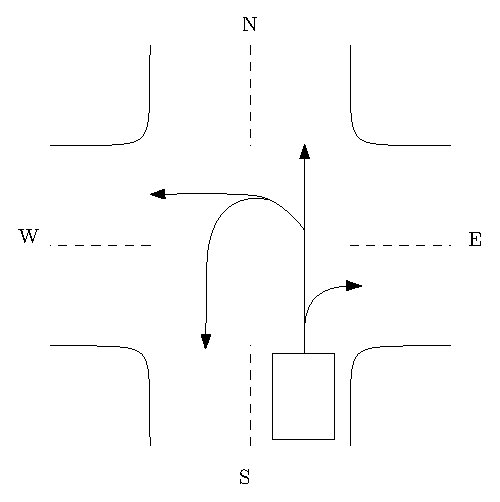
\includegraphics{crossroads}
\label{fig:crossroads}
\caption{Возможные направления движения}
\end{figure}

Сначала смоделируем сам перекресток без каких-либо правил проезда. Интуиция подсказывает, что состояния машины на перекрестке (подъезжает к нему, стоит перед его началом, едет по нему) можно попробовать смоделировать в виде автомата. Для этого воспользуемся нашим шаблоном (итоговая спецификация размещена в Приложении \ref{appendix:crossroads}):

\begin{tla}
---- MODULE crossroads ----
EXTENDS Sequences, Integers, TLC, FiniteSets, Helpers
CONSTANTS Cars

DirsSeq == <<"N", "E", "S", "W">>
Dirs == Range(DirsSeq)
\end{tla}
\begin{tlatex}
\@x{}\moduleLeftDash\@xx{ {\MODULE} crossroads}\moduleRightDash\@xx{}%
\@x{ {\EXTENDS} Sequences ,\, Integers ,\, TLC ,\, FiniteSets ,\, Helpers}%
\@x{ {\CONSTANTS} Cars}%
\@pvspace{8.0pt}%
 \@x{ DirsSeq \.{\defeq} {\langle}\@w{N} ,\,\@w{E} ,\,\@w{S} ,\,\@w{W}
 {\rangle}}%
\@x{ Dirs \.{\defeq} Range ( DirsSeq )}%
\end{tlatex}
\begin{ppcal}
--algorithm crossroadPass
variables
  queue = [d \in Dirs |-> <<>>],

fair process car \in Cars
variables
  from \in Dirs, to \in Dirs, state = "Initial";
begin
  Action:
    either
      await state = "Initial";
      state := "Waiting";
      queue[from] := Append(queue[from], self);
    or
      await state = "Waiting";
      state := "Passing";
    or
      await state = "Passing";
      state := "Initial";
      queue[from] := Tail(queue[from]);
    end either;
    goto Action;
end process;

end algorithm;
\end{ppcal}
\begin{tlatex}
\@x{ {\p@mmalgorithm} crossroadPass}%
\@x{ {\p@variables}}%
 \@x{\@s{8.2} queue \.{=} [ d \.{\in} Dirs \.{\mapsto} {\langle} {\rangle} ]
 ,\,}%
\@pvspace{8.0pt}%
\@x{ {\p@fair} {\p@process} car \.{\in} Cars}%
\@x{ {\p@variables}}%
 \@x{\@s{8.2} from \.{\in} Dirs ,\, to \.{\in} Dirs ,\, state
 \.{=}\@w{Initial} {\p@semicolon}}%
\@x{ {\p@begin}}%
\@x{\@s{8.2} Action\@s{.5}\textrm{:}\@s{3}}%
\@x{\@s{16.4} {\p@either}}%
\@x{\@s{24.59} {\p@await} state \.{=}\@w{Initial} {\p@semicolon}}%
\@x{\@s{24.59} state \.{:=}\@w{Waiting} {\p@semicolon}}%
 \@x{\@s{24.59} queue [ from ] \.{:=} Append ( queue [ from ] ,\, self )
 {\p@semicolon}}%
\@x{\@s{16.4} {\p@or}}%
\@x{\@s{24.59} {\p@await} state \.{=}\@w{Waiting} {\p@semicolon}}%
\@x{\@s{24.59} state \.{:=}\@w{Passing} {\p@semicolon}}%
\@x{\@s{16.4} {\p@or}}%
\@x{\@s{24.59} {\p@await} state \.{=}\@w{Passing} {\p@semicolon}}%
\@x{\@s{24.59} state \.{:=}\@w{Initial} {\p@semicolon}}%
\@x{\@s{24.59} queue [ from ] \.{:=} Tail ( queue [ from ] ) {\p@semicolon}}%
\@x{\@s{16.4} {\p@end} {\p@either} {\p@semicolon}}%
\@x{\@s{16.4} {\p@goto} Action {\p@semicolon}}%
\@x{ {\p@end} {\p@process} {\p@semicolon}}%
\@pvspace{8.0pt}%
\@x{ {\p@end} {\p@algorithm} {\p@semicolon}}%
\end{tlatex}

Направления движения моделируем и как множество \emph{Dirs}, и как последовательность \emph{DirsSeq}. В то время как множество полезно для ветвления алгоритма по всем направлениям, последовательность поможет устанавливать относительность направлений (например ``Проезд из S в E --- поворт направо``).

Подъезжая к перекрестку, машина становится в очередь \emph{queue} на проезд. Чтобы смоделировать непрерывный поток машин по некоторому направлению, после окончания алгоритма делаем \emph{goto} в начальное состояние. Ключевое слово \emph{fair} перед \emph{process} подразумевает, что машины не перестанут двигаться по алгоритму, пока будут доступные шаги.

Пора определить, что такое безопасный перекресток. Будем считать, что перекресток безопасен, если для любой пары машин верно: когда они переезжают перекресток одновременно, их пути не пересекаются, то есть они не могут столкнуться. Рассмотрение всех возможных вариантов столкновения мы пока отложим и остановимся на простом подможестве: машины могут столкнуться, если они едут в одну и ту же полосу.

\begin{tla}
  MkCar(f, t, s) == [from |-> f, to |-> t, state |-> s]

  Crashing(car1, car2) == 
    /\ car1.state = "Passing" 
    /\ car2.state = "Passing" 
    /\ car1.to = car2.to  

  NoCrash == 
    \A c1, c2 \in Cars:
    (c1 /= c2) => ~Crashing(
      MkCar(from[c1], to[c1], state[c1]), 
      MkCar(from[c2], to[c2], state[c2])
    )
\end{tla}
\begin{tlatex}
 \@x{\@s{8.2} MkCar ( f ,\, t ,\, s ) \.{\defeq} [ from \.{\mapsto} f ,\, to
 \.{\mapsto} t ,\, state \.{\mapsto} s ]}%
\@pvspace{8.0pt}%
\@x{\@s{8.2} Crashing ( car1 ,\, car2 ) \.{\defeq}}%
\@x{\@s{16.4} \.{\land} car1 . state \.{=}\@w{Passing}}%
\@x{\@s{16.4} \.{\land} car2 . state \.{=}\@w{Passing}}%
\@x{\@s{16.4} \.{\land} car1 . to \.{=} car2 . to}%
\@pvspace{8.0pt}%
\@x{\@s{8.2} NoCrash \.{\defeq}}%
\@x{\@s{16.4} \A\, c1 ,\, c2 \.{\in} Cars \.{:}}%
\@x{\@s{16.4} ( c1 \.{\neq} c2 ) \.{\implies} {\lnot} Crashing (}%
\@x{\@s{25.98} MkCar ( from [ c1 ] ,\, to [ c1 ] ,\, state [ c1 ] ) ,\,}%
\@x{\@s{25.98} MkCar ( from [ c2 ] ,\, to [ c2 ] ,\, state [ c2 ] )}%
\@x{\@s{16.4} )}%
\end{tlatex}

Пока будем запускать модель для двух потоков машин \emph{c1} и \emph{c2}.
Просим проверщик моделей запуститься с инвариантом \emph{NoCrash} и закономерно получаем историю, которая ему противоречит: к примеру, движения \(S \rightarrow N\) и \(W \rightarrow E\) могут привести к столкновению.

Перед выездом на перекресток добавим проверку \emph{CanMove}, которая реализует известное ``правило правой руки``: нужно уступать дорогу тем, кто справа от нас и чья траектория пересекается с нашей.

\begin{ppcal}
algorithm crossroadPass
variables
  queue = [d \in Dirs |-> <<>>],
  wantTo = [d \in Dirs |-> {}],
  wantFrom = [d \in Dirs |-> {}],
  passing = [d \in Dirs |-> {}];
define
  CanMove(car, from, to) == 
    LET
      Candidates == Heads(queue)
      To(t) == wantTo[t] \intersect Candidates
      From(f) == wantFrom[f] \intersect Candidates
      Reversing(d) == To(d) \intersect From(d) 
      Conflicts(f, t) == ((To(t) \intersect From(RightTo[f])) \ Reversing(t)) \union passing[t]
      Reversal(f, t) == (f = t) => Cardinality(To(t)) = 1 \* reversing car itself
    IN
    car \in Candidates /\
    Cardinality(Conflicts(from, to)) = 0 /\
    Reversal(from, to)
end define;

fair process car \in Cars
variables
  from \in Dirs, to \in Dirs, state = "Initial";
begin
  Action:
    either
      await state = "Initial";
      state := "Waiting";
      queue[from] := Append(queue[from], self);
      wantTo[to] := wantTo[to] \union {self};
      wantFrom[from] := wantFrom[from] \union {self};
    or
      await state = "Waiting";
      await CanMove(self, from, to);
      state := "Passing";
      passing[to] := passing[to] \union {self};
    or
      await state = "Passing";
      state := "Initial";
      queue[from] := Tail(queue[from]);
      wantTo[to] := wantTo[to] \ {self};
      wantFrom[from] := wantFrom[from] \ {self};
      passing[to] := passing[to] \ {self};
    end either;
    goto Action;
end process;

end algorithm;
\end{ppcal}
\begin{tlatex}
\@x{ {\p@algorithm} crossroadPass}%
\@x{ {\p@variables}}%
 \@x{\@s{8.2} queue \.{=} [ d \.{\in} Dirs \.{\mapsto} {\langle} {\rangle} ]
 ,\,}%
\@x{\@s{8.2} wantTo \.{=} [ d \.{\in} Dirs \.{\mapsto} \{ \} ] ,\,}%
\@x{\@s{8.2} wantFrom \.{=} [ d \.{\in} Dirs \.{\mapsto} \{ \} ] ,\,}%
 \@x{\@s{8.2} passing \.{=} [ d \.{\in} Dirs \.{\mapsto} \{ \} ]
 {\p@semicolon}}%
\@x{ {\p@define}}%
\@x{\@s{8.2} CanMove ( car ,\, from ,\, to ) \.{\defeq}}%
\@x{\@s{16.4} \.{\LET}}%
\@x{\@s{24.59} Candidates \.{\defeq} Heads ( queue )}%
\@x{\@s{24.59} To ( t ) \.{\defeq} wantTo [ t ] \.{\cap} Candidates}%
\@x{\@s{24.59} From ( f ) \.{\defeq} wantFrom [ f ] \.{\cap} Candidates}%
\@x{\@s{24.59} Reversing ( d ) \.{\defeq} To ( d ) \.{\cap} From ( d )}%
 \@x{\@s{24.59} Conflicts ( f ,\, t ) \.{\defeq} ( ( To ( t ) \.{\cap} From (
 RightTo [ f ] ) ) \.{\,\backslash\,} Reversing ( t ) ) \.{\cup} passing [ t
 ]}%
 \@x{\@s{24.59} Reversal ( f ,\, t ) \.{\defeq} ( f \.{=} t ) \.{\implies}
 Cardinality ( To ( t ) ) \.{=} 1}%
\@y{%
  reversing car itself
}%
\@xx{}%
\@x{\@s{16.4} \.{\IN}}%
\@x{\@s{16.4} car \.{\in} Candidates \.{\land}}%
\@x{\@s{16.4} Cardinality ( Conflicts ( from ,\, to ) ) \.{=} 0 \.{\land}}%
\@x{\@s{16.4} Reversal ( from ,\, to )}%
\@x{ {\p@end} {\p@define} {\p@semicolon}}%
\@pvspace{8.0pt}%
\@x{ {\p@fair} {\p@process} car \.{\in} Cars}%
\@x{ {\p@variables}}%
 \@x{\@s{8.2} from \.{\in} Dirs ,\, to \.{\in} Dirs ,\, state
 \.{=}\@w{Initial} {\p@semicolon}}%
\@x{ {\p@begin}}%
\@x{\@s{8.2} Action\@s{.5}\textrm{:}\@s{3}}%
\@x{\@s{16.4} {\p@either}}%
\@x{\@s{24.59} {\p@await} state \.{=}\@w{Initial} {\p@semicolon}}%
\@x{\@s{24.59} state \.{:=}\@w{Waiting} {\p@semicolon}}%
 \@x{\@s{24.59} queue [ from ] \.{:=} Append ( queue [ from ] ,\, self )
 {\p@semicolon}}%
 \@x{\@s{24.59} wantTo [ to ] \.{:=} wantTo [ to ] \.{\cup} \{ self \}
 {\p@semicolon}}%
 \@x{\@s{24.59} wantFrom [ from ] \.{:=} wantFrom [ from ] \.{\cup} \{ self \}
 {\p@semicolon}}%
\@x{\@s{16.4} {\p@or}}%
\@x{\@s{24.59} {\p@await} state \.{=}\@w{Waiting} {\p@semicolon}}%
\@x{\@s{24.59} {\p@await} CanMove ( self ,\, from ,\, to ) {\p@semicolon}}%
\@x{\@s{24.59} state \.{:=}\@w{Passing} {\p@semicolon}}%
 \@x{\@s{24.59} passing [ to ] \.{:=} passing [ to ] \.{\cup} \{ self \}
 {\p@semicolon}}%
\@x{\@s{16.4} {\p@or}}%
\@x{\@s{24.59} {\p@await} state \.{=}\@w{Passing} {\p@semicolon}}%
\@x{\@s{24.59} state \.{:=}\@w{Initial} {\p@semicolon}}%
\@x{\@s{24.59} queue [ from ] \.{:=} Tail ( queue [ from ] ) {\p@semicolon}}%
 \@x{\@s{24.59} wantTo [ to ] \.{:=} wantTo [ to ] \.{\,\backslash\,} \{ self
 \} {\p@semicolon}}%
 \@x{\@s{24.59} wantFrom [ from ] \.{:=} wantFrom [ from ] \.{\,\backslash\,}
 \{ self \} {\p@semicolon}}%
 \@x{\@s{24.59} passing [ to ] \.{:=} passing [ to ] \.{\,\backslash\,} \{
 self \} {\p@semicolon}}%
\@x{\@s{16.4} {\p@end} {\p@either} {\p@semicolon}}%
\@x{\@s{16.4} {\p@goto} Action {\p@semicolon}}%
\@x{ {\p@end} {\p@process} {\p@semicolon}}%
\@pvspace{8.0pt}%
\@x{ {\p@end} {\p@algorithm} {\p@semicolon}}%
\end{tlatex}

Такая спецификация удовлетворяет инварианту \emph{NoCrash}! Помимо безопасности естественным свойством перекрестка видится гарантия того, что каждая машина рано или поздно проедет, куда ей нужно. Сформулируем это свойство с помощью темпорального оператора ``когда-нибудь``(\(\Diamond\)).

\begin{tla}
EveryonePasses ==
  \A c \in Cars: <>(state[c] = "Passing")
\end{tla}
\begin{tlatex}
\@x{ EveryonePasses \.{\defeq}}%
 \@x{\@s{8.2} \A\, c \.{\in} Cars \.{:} {\Diamond} ( state [ c ]
 \.{=}\@w{Passing} )}%
\end{tlatex}

Ошибка! Запуск проверки обнаружил историю, в которой машина может бесконечно долго стоять в ожидании своей очереди (Пусть \(c1: S \rightarrow S\) и \(c2: N \rightarrow S\). Если поток машин \emph{c2} непрерывен, машина \emph{c1} будет обречена на вечное ожидание возможности разворота). Очевидно, в реальной жизни не может существовать бесконечного потока машин, однако полученный результат свидетельствует о ситуации на дороге, которую стоит учитывать при проектировании развязок.
 
Вернемся к нашему упрощенному определению столкновения машин и расширим его до всех возможных ситуаций:

\begin{tla}
IndOf(dir) == Matching(DirsSeq, dir)

RightTo[x \in Dirs] == 
  LET RightInd == (IndOf(x) % 4) + 1
  IN DirsSeq[RightInd]
OppTo[x \in Dirs] ==
  LET OppInd == ((IndOf(x) + 1) % 4) + 1
  IN DirsSeq[OppInd]
LeftTo[x \in Dirs] == 
  LET LeftInd == ((IndOf(x) + 2) % 4) + 1
  IN DirsSeq[LeftInd] 

MkCar(f, t, s) == [from |-> f, to |-> t, state |-> s]
Straight(car) == Abs(IndOf(car.from) - IndOf(car.to)) = 2
Left(car) == Abs(IndOf(car.from) - IndOf(car.to)) = 3
Reverse(car) == car.from = car.to
  
Crashing(car1, car2) == 
  /\ car1.state = "Passing" 
  /\ car2.state = "Passing" 
  /\ \/ car1.to = car2.to  
     \/ /\ Straight(car1) 
        /\ \/ car2.from = RightTo[car1.from] 
           \/ Straight(car2)
     \/ /\ Left(car1)
        /\ \/ car2.from = RightTo[car1.from]
           \/ car2.from = OppTo[car1.from]
           \/ /\ car2.from = LeftTo[car1.from]
              /\ Left(car2) \/ Straight(car2)
     \/ /\ Reverse(car1)
\end{tla}
\begin{tlatex}
\@x{ IndOf ( dir ) \.{\defeq} Matching ( DirsSeq ,\, dir )}%
\@pvspace{8.0pt}%
\@x{ RightTo [ x \.{\in} Dirs ] \.{\defeq}}%
\@x{\@s{8.2} \.{\LET} RightInd \.{\defeq} ( IndOf ( x ) \.{\%} 4 ) \.{+} 1}%
\@x{\@s{8.2} \.{\IN} DirsSeq [ RightInd ]}%
\@x{ OppTo [ x \.{\in} Dirs ] \.{\defeq}}%
 \@x{\@s{8.2} \.{\LET} OppInd \.{\defeq} ( ( IndOf ( x ) \.{+} 1 ) \.{\%} 4 )
 \.{+} 1}%
\@x{\@s{8.2} \.{\IN} DirsSeq [ OppInd ]}%
\@x{ LeftTo [ x \.{\in} Dirs ] \.{\defeq}}%
 \@x{\@s{8.2} \.{\LET}\@s{1.59} LeftInd \.{\defeq} ( ( IndOf ( x ) \.{+} 2 )
 \.{\%} 4 ) \.{+} 1}%
\@x{\@s{8.2} \.{\IN} DirsSeq [ LeftInd ]}%
\@pvspace{8.0pt}%
 \@x{ MkCar ( f ,\, t ,\, s ) \.{\defeq} [ from \.{\mapsto} f ,\, to
 \.{\mapsto} t ,\, state \.{\mapsto} s ]}%
 \@x{ Straight ( car ) \.{\defeq} Abs ( IndOf ( car . from ) \.{-} IndOf ( car
 . to ) ) \.{=} 2}%
 \@x{ Left ( car ) \.{\defeq} Abs ( IndOf ( car . from ) \.{-} IndOf ( car .
 to ) ) \.{=} 3}%
\@x{ Reverse ( car ) \.{\defeq} car . from \.{=} car . to}%
\@pvspace{8.0pt}%
\@x{ Crashing ( car1 ,\, car2 ) \.{\defeq}}%
\@x{\@s{8.2} \.{\land} car1 . state \.{=}\@w{Passing}}%
\@x{\@s{8.2} \.{\land} car2 . state \.{=}\@w{Passing}}%
\@x{\@s{8.2} \.{\land} \.{\lor} car1 . to\@s{0.75} \.{=} car2 . to}%
\@x{\@s{24.19} \.{\lor} \.{\land} Straight ( car1 )}%
\@x{\@s{40.19} \.{\land} \.{\lor} car2 . from \.{=} RightTo [ car1 . from ]}%
\@x{\@s{56.19} \.{\lor} Straight ( car2 )}%
\@x{\@s{24.19} \.{\lor} \.{\land} Left ( car1 )}%
\@x{\@s{40.19} \.{\land} \.{\lor} car2 . from \.{=} RightTo [ car1 . from ]}%
\@x{\@s{56.19} \.{\lor} car2 . from \.{=} OppTo [ car1 . from ]}%
\@x{\@s{56.19} \.{\lor} \.{\land} car2 . from \.{=} LeftTo [ car1 . from ]}%
\@x{\@s{72.19} \.{\land} Left ( car2 ) \.{\lor} Straight ( car2 )}%
\@x{\@s{24.19} \.{\lor} \.{\land} Reverse ( car1 )}%
\end{tlatex}

Обновленное условие столкновения дает интересные результат: правило правой руки не помогает в разрешении ситуации \(c1: S \rightarrow S, c2: N \rightarrow N \), то есть когда две машины едут навстречу друг другу и обе хотят развернуться. 


Еще один интересный результат --- обнаружение дедлока в ситуации, когда с разных сторон к перекрестку подъезжают сразу 4 машины с пересекающимися направлениями движения.

В этом примере мы начали со спецификации в одно предложение и пришли к необходимости правил по проезду перекрестка. Замоделировав ``правило правой руки``, выяснили часть его фундаментальных проблем:
\begin{itemize}
  \item При неудачном стечении обстоятельств машины могут никогда не проехать перекресток.
  \item Порядок проезда не определен для встречных разворачивающихся машин. 
  \item Порядок проезда не определен для 4 машин на разных концах перекрестка.
\end{itemize}

Хоть по отдельности такие ситуации могут происходить редко, каждая из них может провоцировать аварийную ситуацию. Поэтому полезно знать о подобных ограничениях при проектировании городских улиц.

\subsection{Запрос цены}

\section{Анализ применимости}
Этот раздел завершает рассказ о методике, приводя рассуждения о накладных расходах ее применения, ее достоинствах и ограничениях.
Все рассуждения выведены эмпирическим путем.

\subsection{Опыт}
Был проведен эксперимент: методика была опробована на практике. Нескольким разработчикам было выделено время на изучение \tlapl и интеграцию в повседневную работу. От старта эксперимента до получения первых полезных спецификаций у разных участников ушло от нескольких дней до двух недель. Разработчики отметили простоту концептов, выразительность языка и возможность переиспользования их опыта программирования. 

Наиболее сложным оказалось формулирование темпоральных свойств. В связи с этим был разработан описанный выше набор вопросов, облегчающих обнаружение инвариантов. Также выяснилось, что качество инструментов для \tlapl уступает качеству оных для языков программирования. Это послужило мотивацией для ряда разработок, о которых речь пойдет в последней главе работы.

Полученные спецификации помогли выявить язъяны в исходном дизайне и подсветить хрупкие места системы. Такие места --- естественный кандидат для мониторинга. Плюс мониторинга, выведенного из спецификации в возможности отслеживания свойства, сформулированных на языке, понятном не только разработчикам.

По итогу эксперимента стали ясны достоинства и ограничения методики, опишем их детальнее.

\subsection{Достоинства}
\begin{itemize}
  \item Проверщик моделей хорошо находят ошибки, проявляющиеся в конкурентном окружении с неопределенным порядком событий.
  \item Процесс спецификации выявляет противоречивость в требованиях и возможную недостижимость (или ограниченную достижимость) желаемых свойств.
  \item Формальные спецификации являются полезным дополнением к документации бизнес-процессов.
  \item Язык \tlapl построен на простых математических концептах (теория множеств, логика предикатов), знакомых многим разработчикам. Это делает его доступным для изучения в отличии от интерактивных доказателей теорем (таких как Coq, Isabelle, и т.д.).
  \item Неожиданным стало наблюдение о том, что накопление опыта формальной верификации смещает парадигму мышления и помогает видеть больше ошибок даже до начала применения методики.
\end{itemize}



\subsection{Ограничения}
Естественно, методика не является ``серебряной пулей`` и перед ее применением необходимо взвесить пользу и затраты от ее применения. Для оценки затрат полезно знать о следующих ограничениях:
\begin{itemize}
  \item Временные затраты.
  \item Соответствие кода и спецификации.
  \item Композируемость спецификаций.
\end{itemize}

Раскроем каждый из пунктов детальнее.


\subsubsection{Временные затраты}
Помимо времени обучения, упомянутое выше, естественным образом увеличится время, уделяемое на этапе спецификации. По наблюдениям того же опыта оно удваивалось по сравнению со специфицированием без применения формальных методов, и помимо аналитиков (бизнес, системных) требовалось привлекать разработчиков.

Таким образом применение методики для краткоживущих или тестовых проектов видится нецелесообразным.

\subsubsection{Соответствие кода и спецификации}
Вопрос генерации по определению корректного кода из формально верифицированных спецификаций --- краеугольный камень формальных методов. На данный момент это является нерешенной задачей и активной темой для исследования. В частности, известны попытки генерации Elixir кода по \tlapl \cite{tlaElixir}. Пока эта проблема остается, у нас нет возможности настроить автоматическую проверку соответствия кода и спецификации. Поэтому мы не застрахованы от ошибок переноса спецификации в код, как и при классическом подходе.

\subsubsection{Композируемость спецификаций}
Интуиция программиста ожидает, что спецификации должны быть организованы как программы: через множество независимых модулей, которые взаимодействуют через публичные интерфейсы и не знают о деталях реализации друг друга. Это более удобочитаемо и переиспользуемо, чем одна большая программа. Модули могут быть протестированы по отдельности и заботиться лишь о том, как их скомбинировать. 

В отличие от программ, большинство спецификаций пишутся в виде одного файла с компонентами, написанными с нуля для каждой спецификации. Могут ли они композироваться так же, как программы? 

По сути, спецификации являются математическими выражениями, и мы пытаемся рассуждать о их свойствах (утверждениях, верных для всех поведений системы). Определим композицию двух спецификаций как их объединение, сохраняющее свойства обеих без необходимости углубления в детали любой из них. Хорошей интуицией здесь может служить композиция функций: если \(f(x)\) имеет сигнатуру типа \(a \rightarrow b\) и \(g(x)\) сигнатуру \(a \rightarrow c\), тогда \(g \circ f = g(f(x))\) имеет сигнатуру \(a \rightarrow c\). Мы знаем, что композиция функций сохраняет безопасность типов без знания начинки любой из функций. Композиция спецификаций желательно должна выглядеть так же: без изменения реализаций можно скомпозировать две спецификации.

Рассмотрим классический пример лампочки. В начальном состоянии либо горит, либо не горит. На следующем шаге состояние инвертируется, процесс выполняется бесконечно:

\begin{tla}
  ---- MODULE Bulb ----
  VARIABLES l1
  Init1 == l1 || !l1
  Switch1 == (l1 => \bigcirc !l1) && (!x => \bigcirc l1)

  Spec1 == Init1 && []Switch1
\end{tla}
\begin{tlatex}
\@x{\@s{8.2}}\moduleLeftDash\@xx{ {\MODULE} Bulb}\moduleRightDash\@xx{}%
\@x{\@s{8.2} {\VARIABLES} l1}%
\@x{\@s{8.2} Init1 \.{\defeq} l1 \.{\p@barbar} {\bang} l1}%
 \@x{\@s{8.2} Switch1 \.{\defeq} ( l1 \.{\implies} \.{\bigcirc} {\bang} l1 )
 \.{\,\&\&\,} ( {\bang} x \.{\implies} \.{\bigcirc} l1 )}%
\@pvspace{8.0pt}%
\@x{\@s{8.2} Spec1 \.{\defeq} Init1 \.{\,\&\&\,} {\Box} Switch1}%
\end{tlatex}

У этого кода лишь два доступных исполнения: чередование начинается с негорящей лампочки или с горящей.

Предпримем попытку композиции спецификации самой с собой для получения двух лампочек:

\begin{tla}
  Spec == Spec1 && Spec2
\end{tla}
\begin{tlatex}
\@x{\@s{8.2} Spec \.{\defeq} Spec1 \.{\,\&\&\,} Spec2}%
\end{tlatex}

Такая композиция гарантирует, что все свойства обеих спецификаций выполнены. Она позволяет четыре возможных исполнения, по одному на каждую пару начальных значения \(l1\) и \(l2\). Однако обе лампочки синхронны при такой композиции. Например, одна не может мигать быстрее другой. Попробуем другой вариант композиции:

\begin{tla}
  Spec == Spec1 || Spec2
\end{tla}
\begin{tlatex}
\@x{\@s{8.2} Spec \.{\defeq} Spec1 \.{\p@barbar} Spec2}%
\end{tlatex}

Но это также не даст желаемого результата: такая композиция делает один из начальных предикатов опциональным, а мы хотим, чтобы они оба были истинны. Оператор \(\.{\,\&\&\,}\) должен применяться к начальным состояниям, а оператор \(||\) только к предикату \(Switch\). 

Поскольку спецификацию приходится разбивать на компоненты, мы лишены простой композиции. В связи с этим спецификации зачастую пишутся с нуля и являются самостоятельными документами.

\chapter{Доработка инструментов \tlapl}
Для применения методики на практике необходимы инструменты разработки. Фундаментально они должны предоставлять следующие возможности:
\begin{itemize}
  \item Редактирование кода
  \item Запуск проверщкика моделей
  \item Представление результатов запуска
\end{itemize}

Хоть эти задачи и решаются стандартным инструментом \tlapl Toolbox, эксперимент выявил, что он значительно уступает в удобстве IDE для языков программирования.

Первая проблема, с которой пришлось столкнуться --- отсутствие какой-либо подсветки синтаксиса для PlusCal, который пишется в многострочных комментариях \tlapl и лежит в основе предложенной методики. 

Вторая --- эргономика использования стандартного инструмента. В нем отсутствует автоматическая трансляция PlusCal кода в \tlapl и работа через диалоговые окна требует значительного количества манипуляций курсором.

В этой главе будут описаны разработки, произведенные для улучшения опыта разработчиков при использовании методики. Сюда вошли описание tree-sitter \cite{treeSitter} грамматики для лучшей подсветки синтаксиса и разработка плагина для редактора Neovim \cite{nvim}

\section{Подсветка синтаксиса}
Подсветка синтаксиса позволяет акцентировать внимание на одинаковых вещах и помогает отличать разные. Проиллюстрировать пользу подсветки синтаксиса просто на примере. Достаточно попробовать найти ромбы сначала на левом изображении, а затем на правом.

\begin{figure}[h]
  \centering
  \begin{subfigure}{\linewidth}
    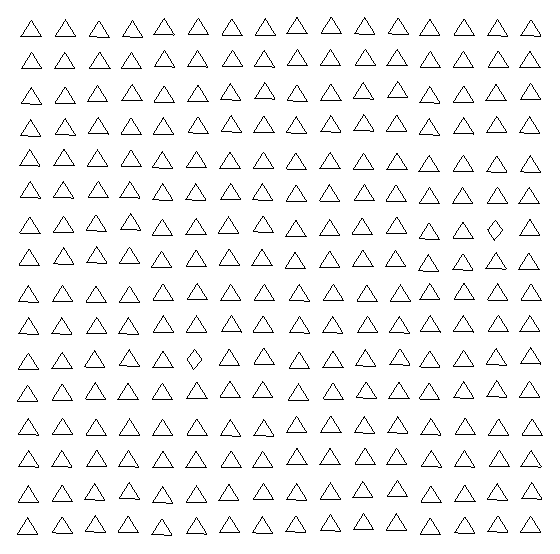
\includegraphics[scale=0.8]{uncolored}\hfill
    
\includegraphics[scale=0.8]{colored}
  \end{subfigure}
  \label{fig:highlighting}
  \caption{Польза подсветки синтаксиса}
\end{figure}

Перенося аналогию на код, с помощью цвета можно отделять, например, литералы и переменные.

Самый простой способ реализации подсветки синтаксиса --- регулярные выражения, которые ищут ключевые слова и последовательности символов. Такой подход прост в реализации, но предоставляет очень ограниченные возможности. Например, он не позволяет делать раскраску в зависимости от контекста, отличать объявления переменных и параметров от ссылок на них, распознавать содержимое коментариев и т.д. Другим подходом является верхнеуровневое описание граммактики языка с помощью парсер-комбинаторов и генерации парсера по этой грамматке. Такой инструментарий предоставляется проектом tree-sitter \cite{treeSitter}. 

Tree-sitter позволяет описывать грамматику с помощью комбинаторов на JavaScript в декларативном стиле. Набор комбинаторов достаточно общий, чтобы описать любой язык с контекстно-свободной грамматикой, а генерируемый парсер инкрементален, что позволяет запускать его на каждое нажатие клавиши. Это делает инструмент пригодным для подсветки синтаксиса (и не только) в текстовых редакторах.

Для описания грамматик доступны следующие основные комбинаторы:
\begin{center}
\begin{tabular}{||c | c||} 
 \hline
Комбинатор & Описание \\ 
 \hline\hline
regexp & Регулярные выражения \\
 \hline
seq(r1, r2) & Последовательность операторов\\ 
 \hline
choice(r1, r2) & Альтернатива операторов \\
 \hline
repeat(r) & Повторение оператора любое число раз\\
 \hline
repeat1(r) & Ненулевое повторение оператора \\
 \hline
optional(r) & Опциональный оператор\\ 
 \hline
\end{tabular}
\end{center}


На момент начала работы грамматика \tlapl уже существовала, однако в ней не хватало значительной части --- грамматики подъязыка PlusCal. Трудности в ее описании связаны с нахождением границ многострочных комментариев, внутри которых находится PlusCal код, транспилируемый в код \tlapl. Многострочные комментарии могут быть вложенными и имеют много граничных случаев с участием специальных символов \(*, (, )\). 

Задача была решена с помощью детерменированного конечного автомата, изображенного на рисунке \ref{fig:blockComment}. Знак \(\char`^\) означает ``не``, \(\backslash s\) означает все пробельные символы, остальные символы используются по своему обычному значению.

\newpage

\begin{figure}[h]
  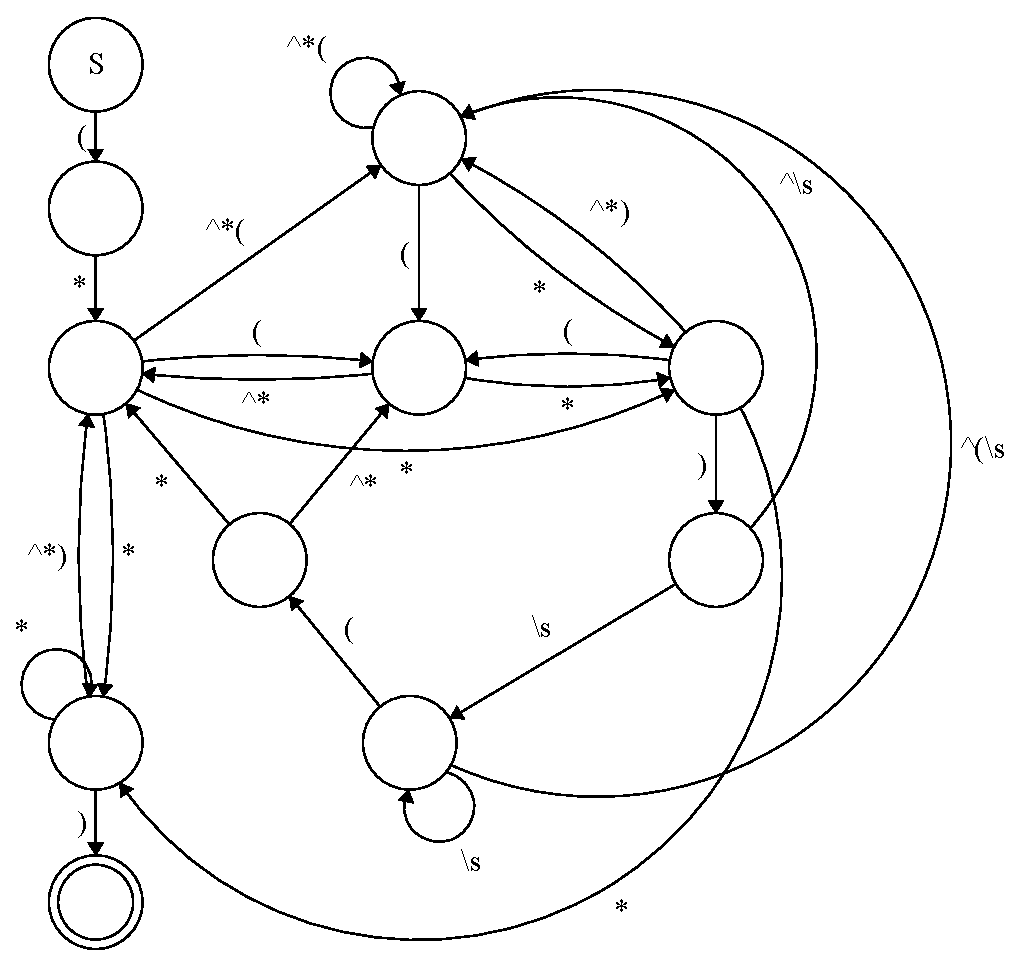
\includegraphics[scale=0.9]{blockComment}
  \caption{Разбор многострочного комментария}
  \label{fig:blockComment}
\end{figure}

После решения задачи о нахождении границ вложенных комментариев дальнейшая реализация грамматики была прямолинейна и велась по официальной ebnf нотации \cite{pcalEbnf}. Были учтены обе разновидности синтаксиса: c-syntax для разработчиков, более знакомых с языком программирования C и p-syntax для разработчико, более знакомых с Python. По завершению работы была дополнена существовавшая грамматика \cite{pcalGrammar}.

Для примера приведем описание одного из правил:

\begin{lstlisting}[label=listing:pcalCSyntax, caption=Правило tree-sitter грамматики для PlusCal C-syntax алгоритма, captionpos=b, style=progStyle]
  _pcal_c_algorithm: $ => seq(
    $.pcal_algorithm_start,
    field('name', $.identifier),
    '{',
    optional($.pcal_var_decls),
    optional(alias($.pcal_c_definitions, $.pcal_definitions)),
    repeat(alias($.pcal_c_macro, $.pcal_macro)),
    repeat(alias($.pcal_c_procedure, $.pcal_procedure)),
    choice(
      alias($.pcal_c_algorithm_body, $.pcal_algorithm_body),
      repeat1(alias($.pcal_c_process, $.pcal_process))
    ),
    '}', $._notify_pcal_algorithm_end
  ),
\end{lstlisting}

Правила описывает верхнеуровневую структуру PlusCal алгоритма, который должен начинаться с конструкции \lstinline[style=progStyle]{--algorithm} и имени алгоритма, затем должны следовать опциональные обхявления переменных, опциональные определения операторов, макросы, процедуры и тело алгоритма.

Полученная грамматика справляется со вложенными многострочными комментариями:

\begin{figure}[h]
  \centering
  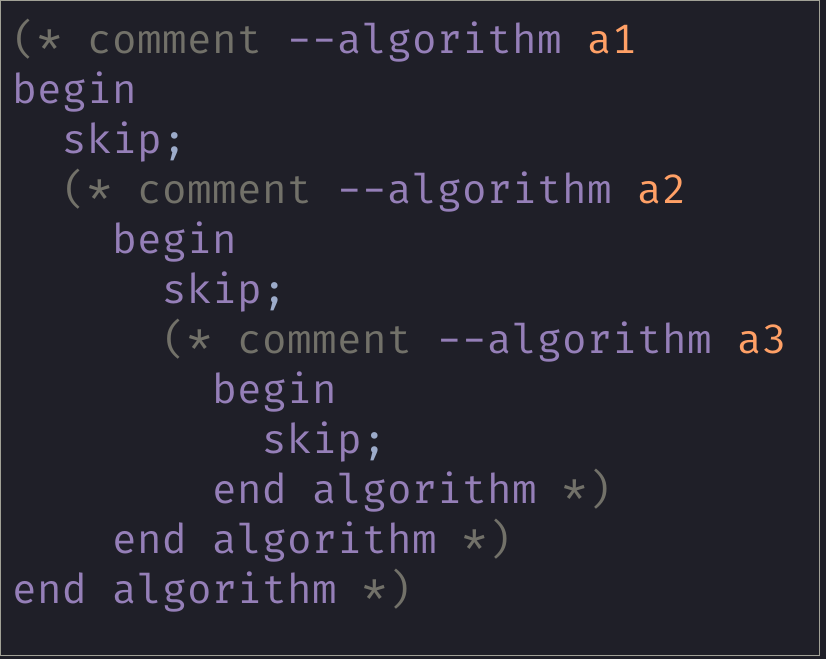
\includegraphics[scale=0.44]{nestedPcal}
  \caption{Вложенные многострочные комментарии \tlapl}
  \label{fig:nestedPcal}
\end{figure}

Для наглядности можно провести сравнение подсветки, основанной на регулярных выражениях (слева) с подсветкой, основанной на полученной грамматике (справа):

\begin{figure}[h]
  \centering
  \begin{subfigure}{\linewidth}
    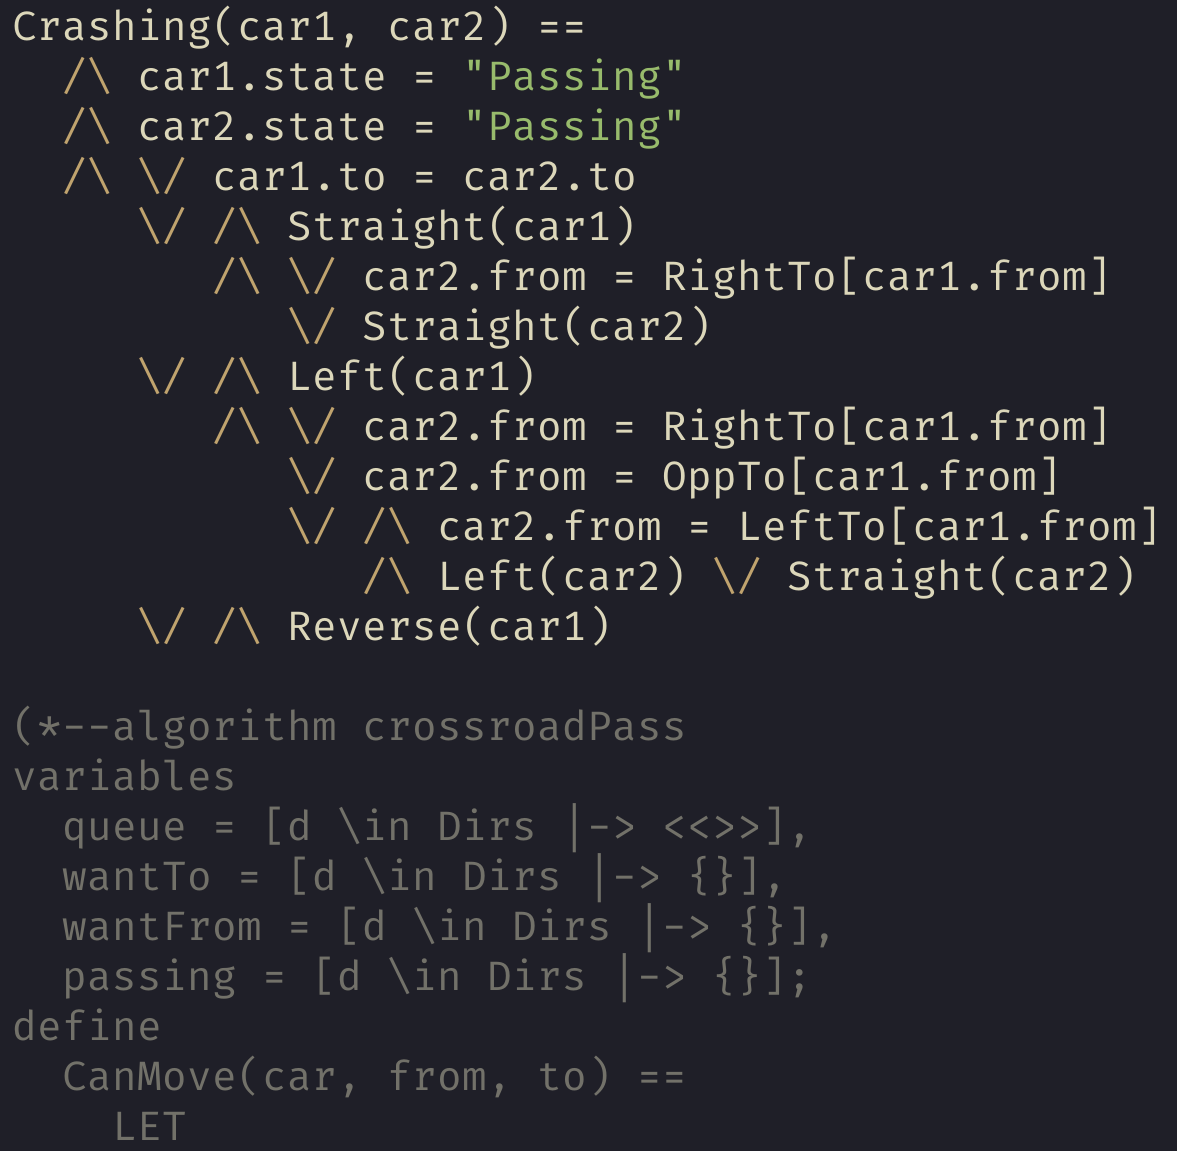
\includegraphics[scale=0.2]{regexHighlight}\hfill
    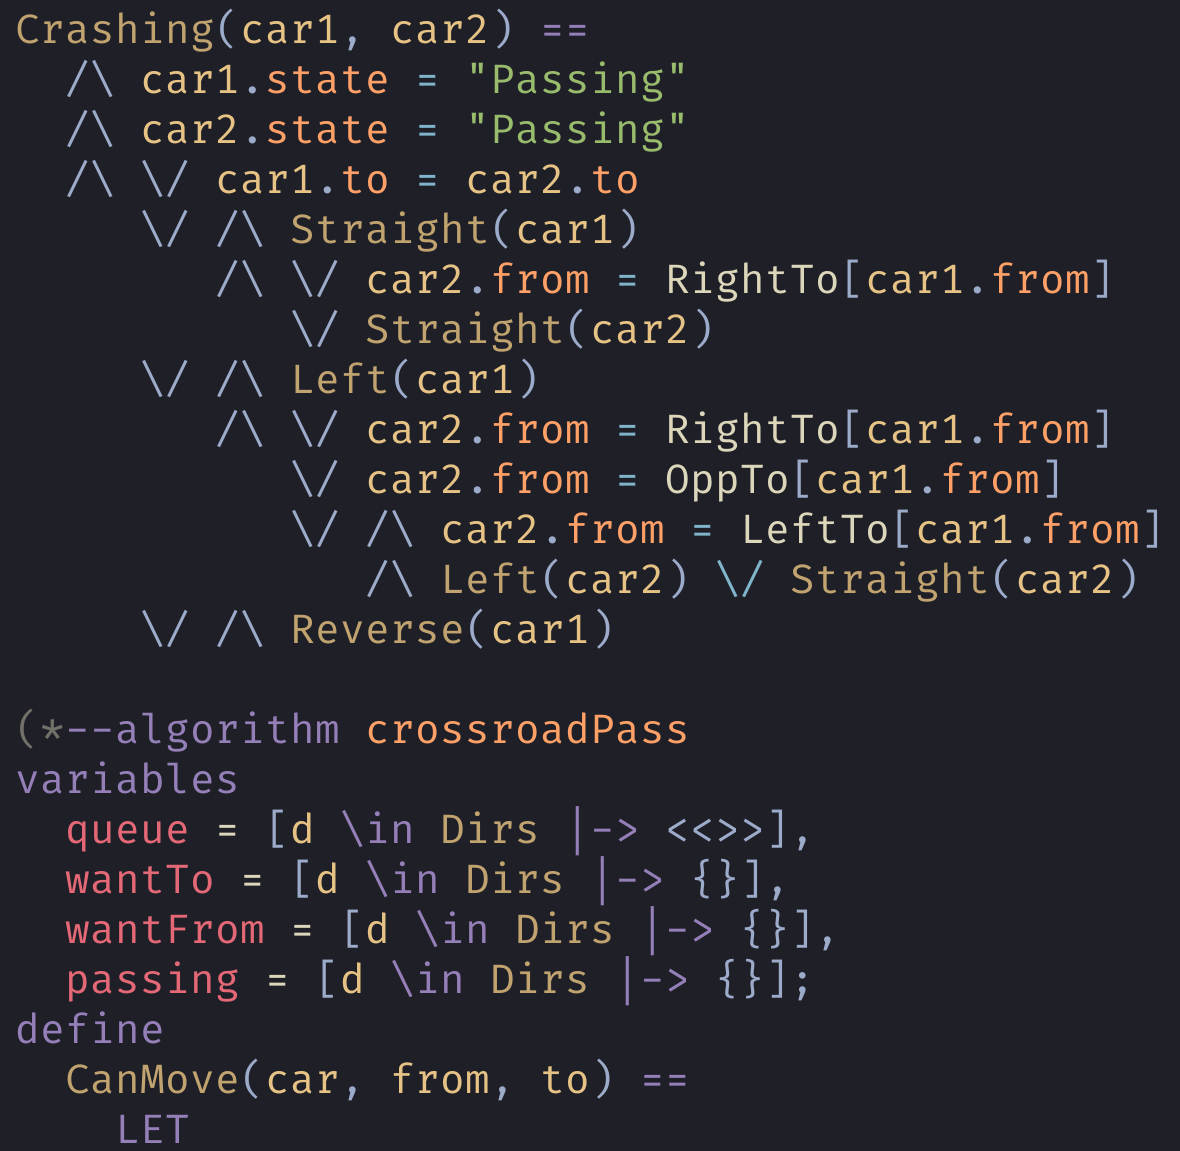
\includegraphics[scale=0.2]{grammarHighlight}
  \end{subfigure}
  \label{fig:highlightingComp}
  \caption{Сравнение подсветок по регулярным выражениям и грамматике}
\end{figure}

На момент написания грамматика доступна для подсветки синтаксиса \tlapl в текстовых редакторах \lstinline[style=progStyle]{Neovim, Emacs, Atom}, а также на \lstinline[style=progStyle]{GitHub}.

Помимо подсветки синтаксиса грамматика открывает возможности для реализации такого функционала как: сворачивание блоков кода, рефактотинги (в т.ч. переименования), а также навигацию при помощи перехода к определению и ссылкам на определение.

\newpage

\section{Плагин для Neovim}

Для применения методики был разработан \lstinline[style=progStyle]{NeoVim}-плагин \cite{tlaNvim}. В него вошел следующий функционал:

\begin{itemize}
  \item Установка инструментов.
  \item Трансляция PlusCal в \tlapl.
  \item Запуск проверщика моделей.
  \item Отображение результатов проверки.
  \item Генерация графа состояний.
  \item Шаблоны кода.
  \item Диагностки LSP.
  \item REPL.
  \item Генерация PDF.
\end{itemize}

Плагин написан на языке программирования \lstinline[style=progStyle]{Lua}, встроенный в редактор. Далее описываются решения, принятые при реализации перечисленных возможностей.

\subsubsection{Установка инструментов}
Стандартные инструменты для работы с \tlapl кодом включают в себя 
\begin{itemize}
  \item Проверщик моделей.
  \item Транслятор PlusCal.
  \item Конвертор пространства состояний в dot-формат.
  \item Конвертор в pdf.
  \item Интерактивный вычислитель выражений, REPL (анг. read-eval-print-loop).
\end{itemize}
Поставляются они в виде единого jar-файла через релизы платформы GitHub. Это накладывает требования на установку виртуальной машины java для пользования плагином. 

Реализована команда \prog{TlaInstall}, которая скачивает инструменты нужной версии и сохраняет для дальнейшего использования. Если инструменты уже были установлены, старая версия перезаписывается.

\subsubsection{Трансляция PlusCal в \tlapl}
Поскольку код PlusCal не может быть проверен TLC напрямую, необходима его трансляция в \tlapl. Этот функционал реализуется командой плагина \prog{TlaTranslate}. 

Для удобства можно воспользоваться механизмом автокоманд и зарегистрировать трансляцию на каждое сохранение файла:
\begin{lstlisting}[label=listing:pcalAutocmd, caption=Автоматическая трансляция PlusCal, captionpos=b, style=progStyle]
  local group = vim.api.nvim_create_augroup(
    "pcal2tla",
    { clear = true }
  )
  vim.api.nvim_create_autocmd(
    "BufWritePre",
    { command = "TlaTranslate", group = "pcal2tla" }
  )
\end{lstlisting}

\subsubsection{Запуск проверщика моделей}
Проверщик моделей TLC требует на вход .tla файл с описанием модели и .cfg файл с указанием ограничений на пространство перебора, а также проверяемыми инвариантами и свойствами. Запуск производится командой \prog{TlaCheck}, которая открывает соседнее вертикальное окно и транслирует туда преобразованный вывод проверщика.

Для простоты по умолчанию используется файл конфигурации с таким же названием, как и название файла с моделью. Однако это поведение может быть переопределено.

\subsubsection{Отображение результатов проверки}
Вывод TLC состоит из набора сообщений определенного формата. Сообщения возникают по мере прохождения проверки. Также по мере их появления просиходит их разбор и отображения на специальном экране результатов.

Результаты содержат ссылки на код модели. Ссылки реализованы через механизм \prog{ctags} с созданием вспомогательных временных файлов, хранящих соответствие тегов и ссылок на конкретные места в исходных файлах.

\subsubsection{Генерация графа состояний}
Поскольку проверка основыывается на обходе графа состояний в ширину (или в глубину, в зависимости от настройки), этот граф можно визуализировать. Для визуализации графов хорошо подходит специализированный инструмент \prog{dot}, который генерирует изображение по текстовому описанию графа в определенном формате. Стандартные инструменты \tlapl дают возможность вывода графа состояний в этом формате. В плагине за это отвечает команда \prog{TlaToDot}.

\subsubsection{Шаблоны кода}
Интегрированные среды разработки (анг. IDE) получили свое распространение среди разработчиков во многом благодаря наличию подсказок с автодополнением. Для реализации подсказок, учитывающих кодовую базу, необходимы комплексные инструменты вроде языковых серверов (анг. Language Server), однако подсказки для стандартных конструкций языка могут быть реализованы с помощью механизма отрывков (анг. snippets), которые срабатывает на сочетания клавиш или при наборе определенных символов. Такие отрывки реализованы в плагини через интеграцию со сторонним плагином отрывков \prog{luasnip}.

\subsubsection{Диагностки}
Для продуктивного написания кода необходим быстрый цикл обратной связи по синтаксическим ошибкам. Неожиданным помощником в этом стала подсветка синтаксиса по грамматике: нераскрашенный код означает ошибку парсинга, которая свидетельствует о синтаксических ошибках. Однако такой способ не указывает на точную причину проблемы, в связи с этим необходимы диагностики от стороннего инструмента. Таковым является парсер SANY, который также входит в стандартную поставку \tlapl. Реализация диагностик на базе SANY находится в стадии разработки на момент написания.

\subsubsection{REPL}
REPL(read-eval-print-loop) --- интерактивная консоль для вычисления выражений. Такая консоль бывает полезна для проведения быстрых экспериментов при разработке. Плагин предоставляет команду \prog{TlaRepl}, которая запускает новую сессию консоли в текущем окне редактора. На текущий момент функционал REPL ограничен стандартными модулями языка и не позволяет экспериментировать с самописными расширениями.

\subsubsection{Генерация PDF}
\tlapl хорошо подходит для интеграции в математические статьи за счет нативной интеграции с latex. PDF-документы, полученные в итоге, могут быть использованы в качестве документации. Команда плагина \prog{TlaToPdf} исполняет преобразование модели \tlapl в PDF с таким же названием.

\subsubsection{Команды плагина}
В сводной таблице представлены vim-команды, предоставляемые плагином:

\begin{center}
\begin{tabular}{||c |  c||} 
 \hline
 Команда & Описание\\ 
 \hline\hline
 \prog{TlaInstall} & Установка нужной  версии инструментов \tlapl \\
 \hline
 \prog{TlaTranslate} & Трансляция PlusCal кода текущего файла в \tlapl\\
 \hline
 \prog{TlaCheck} & Запуск проверщика моделей TLC с указанной конфигурацией \\
 \hline
 \prog{TlaRepl} & Запуск интерактивной сессии \\
 \hline
 \prog{TlaToDot} & Конвертация графа состояний в dot-формат\\
 \hline
 \prog{TlaToPdf} & Конвертация модели в PDF\\
 \hline
\end{tabular}
\end{center}


\chapter{Выводы}
Цель данной работы состояла в исследовании возможности применимости формальных методов для снижения числа ошибок спецификации в условиях продуктовой разработки. В результатые были опробованы два формальных подхода: доказательство теорем и проверка моделей. 

Проверка моделей на базе языка спецификаций \tlapl показала свою быструю усвояемость. Была разработана методика по применению выбранного языка. В методику вошли рекомендации по уточнению требуемых свойств специфицируемых бизнес-процессом, шаблоны для однопроцессных и многопроцессных алгоритмов, а также автоматов состояний. Методика доказала свою применимость на практике, были оценены ее достоинства, ограничения и затраты на применение. Среди достоинств выделяются эффективное обнаружение ошибок спецификации в конкуррентных средах исполнения, а также выявление противоречий и возможной недостижимости исходных требований. Среди ограничений основными являются невозможность отслеживания соответствии кода и его формальной спецификации, а также отсутсвие композируемости спецификаций.

Помимо методики значимым результатом работы стала доработка инструментов \tlapl: разработка грамматики на базе tree-sitter сделала возможной подсветку синтаксиса в ряде популярных текстовых редакторах и платформе GitHub, а создание Neovim-плагина снабдило процесс написания спецификаций некоторыми возможностями интегрированных сред разработки.

Первичный успех применения методики и улучшение инструментов разработки являются заделом на будущее распространение подхода формальных методов в продуктовой разработки.

\bibliographystyle{unsrt}
\bibliography{references}

\chapter{Приложения}
\refstepcounter{appendix}\label{appendix:crossroads}
\section*{Приложение A. \tlapl примера Перекресток}
\addcontentsline{toc}{subsection}{Приложение A. \tlapl примера Перекресток }

\begin{tla}
  ---- MODULE crossroads ----
EXTENDS Sequences, Integers, TLC, FiniteSets, Helpers
CONSTANTS Cars

DirsSeq == <<"N", "E", "S", "W">>
IndOf(dir) == Matching(DirsSeq, dir)

Dirs == Range(DirsSeq)
RightTo[x \in Dirs] == 
  LET RightInd == (IndOf(x) % 4) + 1
  IN DirsSeq[RightInd]
OppTo[x \in Dirs] ==
  LET OppInd == ((IndOf(x) + 1) % 4) + 1
  IN DirsSeq[OppInd]
LeftTo[x \in Dirs] == 
  LET LeftInd == ((IndOf(x) + 2) % 4) + 1
  IN DirsSeq[LeftInd] 

MkCar(f, t, s) == [from |-> f, to |-> t, state |-> s]
Straight(car) == Abs(IndOf(car.from) - IndOf(car.to)) = 2
Left(car) == Abs(IndOf(car.from) - IndOf(car.to)) = 3
Reverse(car) == car.from = car.to
  
Crashing(car1, car2) == 
  /\ car1.state = "Passing" 
  /\ car2.state = "Passing" 
  /\ \/ car1.to = car2.to  
     \/ /\ Straight(car1) 
        /\ \/ car2.from = RightTo[car1.from] 
           \/ Straight(car2)
     \/ /\ Left(car1)
        /\ \/ car2.from = RightTo[car1.from]
           \/ car2.from = OppTo[car1.from]
           \/ /\ car2.from = LeftTo[car1.from]
              /\ Left(car2) \/ Straight(car2)
     \/ /\ Reverse(car1)     
\end{tla}
\begin{tlatex}
\@x{\@s{8.2}}\moduleLeftDash\@xx{ {\MODULE} crossroads}\moduleRightDash\@xx{}%
\@x{ {\EXTENDS} Sequences ,\, Integers ,\, TLC ,\, FiniteSets ,\, Helpers}%
\@x{ {\CONSTANTS} Cars}%
\@pvspace{8.0pt}%
 \@x{ DirsSeq \.{\defeq} {\langle}\@w{N} ,\,\@w{E} ,\,\@w{S} ,\,\@w{W}
 {\rangle}}%
\@x{ IndOf ( dir ) \.{\defeq} Matching ( DirsSeq ,\, dir )}%
\@pvspace{8.0pt}%
\@x{ Dirs \.{\defeq} Range ( DirsSeq )}%
\@x{ RightTo [ x \.{\in} Dirs ] \.{\defeq}}%
\@x{\@s{8.2} \.{\LET} RightInd \.{\defeq} ( IndOf ( x ) \.{\%} 4 ) \.{+} 1}%
\@x{\@s{8.2} \.{\IN} DirsSeq [ RightInd ]}%
\@x{ OppTo [ x \.{\in} Dirs ] \.{\defeq}}%
 \@x{\@s{8.2} \.{\LET} OppInd \.{\defeq} ( ( IndOf ( x ) \.{+} 1 ) \.{\%} 4 )
 \.{+} 1}%
\@x{\@s{8.2} \.{\IN} DirsSeq [ OppInd ]}%
\@x{ LeftTo [ x \.{\in} Dirs ] \.{\defeq}}%
 \@x{\@s{8.2} \.{\LET}\@s{1.59} LeftInd \.{\defeq} ( ( IndOf ( x ) \.{+} 2 )
 \.{\%} 4 ) \.{+} 1}%
\@x{\@s{8.2} \.{\IN} DirsSeq [ LeftInd ]}%
\@pvspace{8.0pt}%
 \@x{ MkCar ( f ,\, t ,\, s ) \.{\defeq} [ from \.{\mapsto} f ,\, to
 \.{\mapsto} t ,\, state \.{\mapsto} s ]}%
 \@x{ Straight ( car ) \.{\defeq} Abs ( IndOf ( car . from ) \.{-} IndOf ( car
 . to ) ) \.{=} 2}%
 \@x{ Left ( car ) \.{\defeq} Abs ( IndOf ( car . from ) \.{-} IndOf ( car .
 to ) ) \.{=} 3}%
\@x{ Reverse ( car ) \.{\defeq} car . from \.{=} car . to}%
\@pvspace{8.0pt}%
\@x{ Crashing ( car1 ,\, car2 ) \.{\defeq}}%
\@x{\@s{8.2} \.{\land} car1 . state \.{=}\@w{Passing}}%
\@x{\@s{8.2} \.{\land} car2 . state \.{=}\@w{Passing}}%
\@x{\@s{8.2} \.{\land} \.{\lor} car1 . to\@s{0.75} \.{=} car2 . to}%
\@x{\@s{24.19} \.{\lor} \.{\land} Straight ( car1 )}%
\@x{\@s{40.19} \.{\land} \.{\lor} car2 . from \.{=} RightTo [ car1 . from ]}%
\@x{\@s{56.19} \.{\lor} Straight ( car2 )}%
\@x{\@s{24.19} \.{\lor} \.{\land} Left ( car1 )}%
\@x{\@s{40.19} \.{\land} \.{\lor} car2 . from \.{=} RightTo [ car1 . from ]}%
\@x{\@s{56.19} \.{\lor} car2 . from \.{=} OppTo [ car1 . from ]}%
\@x{\@s{56.19} \.{\lor} \.{\land} car2 . from \.{=} LeftTo [ car1 . from ]}%
\@x{\@s{72.19} \.{\land} Left ( car2 ) \.{\lor} Straight ( car2 )}%
\@x{\@s{24.19} \.{\lor} \.{\land} Reverse ( car1 )}%
\end{tlatex}
\begin{ppcal}
--algorithm crossroadPass
variables
  queue = [d \in Dirs |-> <<>>],
  wantTo = [d \in Dirs |-> {}],
  wantFrom = [d \in Dirs |-> {}],
  passing = [d \in Dirs |-> {}];
define
  CanMove(car, from, to) == 
    LET
      Candidates == Heads(queue)
      To(t) == wantTo[t] \intersect Candidates
      From(f) == wantFrom[f] \intersect Candidates
      Reversing(d) == To(d) \intersect From(d) 
      Conflicts(f, t) == ((To(t) \intersect From(RightTo[f])) \ Reversing(t)) \union passing[t]
      Reversal(f, t) == (f = t) => Cardinality(To(t)) = 1 \* reversing car itself
    IN
    car \in Candidates /\
    Cardinality(Conflicts(from, to)) = 0 /\
    Reversal(from, to)
end define;

fair process car \in Cars
variables
  from \in Dirs, to \in Dirs, state = "Initial";
begin
  Action:
    either
      await state = "Initial";
      state := "Waiting";
      queue[from] := Append(queue[from], self);
      wantTo[to] := wantTo[to] \union {self};
      wantFrom[from] := wantFrom[from] \union {self};
    or
      await state = "Waiting";
      await CanMove(self, from, to);
      state := "Passing";
      passing[to] := passing[to] \union {self};
    or
      await state = "Passing";
      state := "Initial";
      queue[from] := Tail(queue[from]);
      wantTo[to] := wantTo[to] \ {self};
      wantFrom[from] := wantFrom[from] \ {self};
      passing[to] := passing[to] \ {self};
    end either;
    goto Action;
end process;
end algorithm;
\end{ppcal}
\begin{tlatex}
\@x{ {\p@mmalgorithm} crossroadPass}%
\@x{ {\p@variables}}%
 \@x{\@s{8.2} queue \.{=} [ d \.{\in} Dirs \.{\mapsto} {\langle} {\rangle} ]
 ,\,}%
\@x{\@s{8.2} wantTo \.{=} [ d \.{\in} Dirs \.{\mapsto} \{ \} ] ,\,}%
\@x{\@s{8.2} wantFrom \.{=} [ d \.{\in} Dirs \.{\mapsto} \{ \} ] ,\,}%
 \@x{\@s{8.2} passing \.{=} [ d \.{\in} Dirs \.{\mapsto} \{ \} ]
 {\p@semicolon}}%
\@x{ {\p@define}}%
\@x{\@s{8.2} CanMove ( car ,\, from ,\, to ) \.{\defeq}}%
\@x{\@s{16.4} \.{\LET}}%
\@x{\@s{24.59} Candidates \.{\defeq} Heads ( queue )}%
\@x{\@s{24.59} To ( t ) \.{\defeq} wantTo [ t ] \.{\cap} Candidates}%
\@x{\@s{24.59} From ( f ) \.{\defeq} wantFrom [ f ] \.{\cap} Candidates}%
\@x{\@s{24.59} Reversing ( d ) \.{\defeq} To ( d ) \.{\cap} From ( d )}%
 \@x{\@s{24.59} Conflicts ( f ,\, t ) \.{\defeq} ( ( To ( t ) \.{\cap} From (
 RightTo [ f ] ) ) \.{\,\backslash\,} Reversing ( t ) ) \.{\cup} passing [ t
 ]}%
 \@x{\@s{24.59} Reversal ( f ,\, t ) \.{\defeq} ( f \.{=} t ) \.{\implies}
 Cardinality ( To ( t ) ) \.{=} 1}%
\@y{%
  reversing car itself
}%
\@xx{}%
\@x{\@s{16.4} \.{\IN}}%
\@x{\@s{16.4} car \.{\in} Candidates \.{\land}}%
\@x{\@s{16.4} Cardinality ( Conflicts ( from ,\, to ) ) \.{=} 0 \.{\land}}%
\@x{\@s{16.4} Reversal ( from ,\, to )}%
\@x{ {\p@end} {\p@define} {\p@semicolon}}%
\@pvspace{8.0pt}%
\@x{ {\p@fair} {\p@process} car \.{\in} Cars}%
\@x{ {\p@variables}}%
 \@x{\@s{8.2} from \.{\in} Dirs ,\, to \.{\in} Dirs ,\, state
 \.{=}\@w{Initial} {\p@semicolon}}%
\@x{ {\p@begin}}%
\@x{\@s{8.2} Action\@s{.5}\textrm{:}\@s{3}}%
\@x{\@s{16.4} {\p@either}}%
\@x{\@s{24.59} {\p@await} state \.{=}\@w{Initial} {\p@semicolon}}%
\@x{\@s{24.59} state \.{:=}\@w{Waiting} {\p@semicolon}}%
 \@x{\@s{24.59} queue [ from ] \.{:=} Append ( queue [ from ] ,\, self )
 {\p@semicolon}}%
 \@x{\@s{24.59} wantTo [ to ] \.{:=} wantTo [ to ] \.{\cup} \{ self \}
 {\p@semicolon}}%
 \@x{\@s{24.59} wantFrom [ from ] \.{:=} wantFrom [ from ] \.{\cup} \{ self \}
 {\p@semicolon}}%
\@x{\@s{16.4} {\p@or}}%
\@x{\@s{24.59} {\p@await} state \.{=}\@w{Waiting} {\p@semicolon}}%
\@x{\@s{24.59} {\p@await} CanMove ( self ,\, from ,\, to ) {\p@semicolon}}%
\@x{\@s{24.59} state \.{:=}\@w{Passing} {\p@semicolon}}%
 \@x{\@s{24.59} passing [ to ] \.{:=} passing [ to ] \.{\cup} \{ self \}
 {\p@semicolon}}%
\@x{\@s{16.4} {\p@or}}%
\@x{\@s{24.59} {\p@await} state \.{=}\@w{Passing} {\p@semicolon}}%
\@x{\@s{24.59} state \.{:=}\@w{Initial} {\p@semicolon}}%
\@x{\@s{24.59} queue [ from ] \.{:=} Tail ( queue [ from ] ) {\p@semicolon}}%
 \@x{\@s{24.59} wantTo [ to ] \.{:=} wantTo [ to ] \.{\,\backslash\,} \{ self
 \} {\p@semicolon}}%
 \@x{\@s{24.59} wantFrom [ from ] \.{:=} wantFrom [ from ] \.{\,\backslash\,}
 \{ self \} {\p@semicolon}}%
 \@x{\@s{24.59} passing [ to ] \.{:=} passing [ to ] \.{\,\backslash\,} \{
 self \} {\p@semicolon}}%
\@x{\@s{16.4} {\p@end} {\p@either} {\p@semicolon}}%
\@x{\@s{16.4} {\p@goto} Action {\p@semicolon}}%
\@x{ {\p@end} {\p@process} {\p@semicolon}}%
\@x{ {\p@end} {\p@algorithm} {\p@semicolon}}%
\end{tlatex}

\section*{Приложение B. }

\end{document}

